\chapter{基于双通道注意力的极化信息提取方法}
\section{引言}
极化SAR通过发射、接收不同极化方式的电磁波信息,实现对地物目标散射信息的探测。以水平、垂直两种极化方式接收目标的散射回波可以得到包含目标散射特性的散射矩阵。对散射矩阵进一步解析,使用不同的物理含义的散射基进行分解,可以得到代表不同散射意义的目标分解特征。如何挖掘极化SAR数据中的潜在极化信息,一直是遥感探测领域的难点与重点。通过适合于极化SAR数据特性的特征提取技术,使极化特征具有良好的类内相聚、类间远离的可分性,提升系统对目标特性的感知能力,使极化SAR目标分类任务中的关键步骤。

根据文献\cite{刘高峰2014极化,1017062722.nh},没有一个单一特征能在所有分类中均取得完美的表现,每个方法提取的特征具有其长处以及特征见具有互补性。合理设计极化信息提取方法,综合利用不同类型极化特征的有效信息,理论上能大幅度提升目标的特征表征能力,改善分类结果。现有的极化信息利用研究中,主要存在以下问题:一,目前绝大多数的极化SAR分类方法直接采用相干矩阵作为输入,忽略了目标分解特征的表示方式\citing{zhou2016polarimetric,liu2018polarimetric}。二,直接堆叠所有的极化特征作为输入导致信息冗余且计算量大,甚至降低分类准确度\citing{ren2021mutual}。

本章讨论多类型极化特征信息提取方法,提出了提出了一种基于注意力机制的极化信息提取方法。该方法以注意力机制方法为基础,利用极化散射特征与极化目标分解特征之间的差异性,构建两种类型特征之间融合表征关系,增强极化信息的表征性能,进而提升下游分类任务的准确率。通过两组真实极化SAR数据验证本方法的有效性与优越性。

% 鉴于不同的散射目标之间的散射特性存在差异,引入了关联注意力机制,联合不同层次的极化特征的关系进行联合建模。首先,为了提取不同层次的极化信息,设计了双通道注意力的极化信息提取网络结构,分别对应目标分解通道和散射数据通道。然后,在两个通道中分别利用空间、通道注意力机制,捕捉各自的关键信息。为了挖掘不同层次极化信息的联系,设计了权重融合模块,用于相互引导修正两个通道的注意力权重。最后,结合跨空间学习模块,对不同尺度的极化特征进行再次融合,得到有效的极化特征表示,结合后续的卷积网络与分类器完成目标分类任务。本章提出的双通道注意力的极化信息提取方法,可以作为一个即插即用的插件式组件,应用到现有的任意一个极化SAR目标分类网络中,增强极化信息的表征能力,提高最终的分类准确率。


% 在上一章中,介绍了目标的散射信息可通过极化散射矩阵$S$进行表示,并通过对$S$进行矢量化分解,可以得到极化信息的进一步表征,包括极化相干矩阵$T$和极化协方差矩阵$C$。使用不同的散射基对$T$或$S$进行分解,得到具有不同物理含义的散射分量。在当前的极化SAR目标分类任务中,基于卷积神经网络(CNN)的分类器通常直接采用协方差矩阵和相干矩阵作为输入,而忽略了极化目标分解的特征表示方式\citing{}。在使用CNN进行分类时,由于其分层特征提取特性,前端网络提取的特征层次相对较低,可能未能充分提取极化SAR数据中的有用信息。同时,如果直接堆叠使用所有极化特征作为输入可能导致特征维度的大幅增加,并且多维特征之间必然存在着信息冗余,可能降低分类准确性\citing{}。

% 针对上述问题,本章研究了一种基于双通道注意力机制的极化信息提取方法。该方法以注意力机制为基础,设计双通道的联合注意力结构,联合不同层次的极化特征进行建模,通过两个单独注意力通道提取不同层次的极化特征并相互校正,最终得到可鉴别极化特征。


\section{注意力机制介绍}
\label{sec:sce3_1}
注意力机制是机器学习和深度学习中一种关键的技术,其主要目标是在处理信息是实现对输入数据的加权关注,以便网络模型能够更有效地捕捉与任务相关的信息。基于注意力机制的信息提取在自然语言处理、计算机视觉等领域获得了广泛的应用\citing{hu2018squeeze,vaswani2017attention}。注意力机制使用不同的权重来表示输入特征的不同的重要程度,根据关注的角度差异,可以分为通道注意力、空间注意力和混合注意力三种类型。
\subsection{通道注意力机制}
输入深度网络的特征一般使用多维数据表示,通道注意力专注于挖掘不同通道间的关键,通过自适应地调整通道之间的权重,使网络模型能够更加聚焦于对后续任务有益的特征通道,从而提升模型的性能和泛化能力。压缩和激励网络(Squeeze-and-Extraction Networks, SENet)\citing{hu2018squeeze}是最具代表性的通道注意力实现模型。图\ref{SENet}为SENet的组成结构图,该方法由压缩和激励两个阶段构成。在压缩阶段,通过全局池化操作对输入多维特征进行压缩,将每个通道的信息整合成单一的数值,用于全局感受野的建模。对于维数是$H\times W \times C$的输入特征,压缩操作将其压缩为$1 \times 1 \times C$维,具体如下式所示:
\begin{equation}
  z_c=\mathbf{F}_{sq}\left( \mathbf{u}_c \right) =\frac{1}{H\times W}\sum_{i=1}^H{\sum_{j=1}^W{u\left( i,j \right)}}
\end{equation}

在激励阶段,利用全连接层和激活函数,学习得到每个通道的权重。得到的权重向量用来对原始输入特征图中的每个通道进行加权,形成加权的特征图。具体如下式所示:
\begin{equation}
  \mathbf{s}=\mathbf{F}_{ex}\left( \mathbf{z},\mathbf{W} \right) =\sigma \left( g\left( \mathbf{z},\mathbf{W} \right) \right) =\sigma \left( \mathbf{W}_2\sigma *\left( \mathbf{W}_1\mathbf{z} \right) \right)
\end{equation}
其中,$\sigma$表示ReLu激活函数\citing{nair2010rectified},$W_1 \in \mathbb{R}^{\frac{C}{r}\times C}$且$W_2 \in \mathbb{R}^{C \times \frac{C}{r}}$。

模型最终通过权重向量$s$来对输入进行重标定得到:
\begin{equation}
  \widetilde{\mathbf{x}}_c=F_{scale}\left( \mathbf{u}_c,s_c \right) =s_c\mathbf{u}_c
\end{equation}
其中,$ \widetilde{\mathbf{X}}=\left[ \widetilde{\mathbf{x}_1},\widetilde{\mathbf{x}_2},\cdots ,\widetilde{\mathbf{x}_C} \right] $, $F_{scale}\left( \mathbf{u}_c,s_c \right)$ 表示 $s_c$与特征图$\mathbf{u}_c \in \mathbb{R}^{H\times W}$的通道级乘积。


\begin{figure}[h]
  \centering
  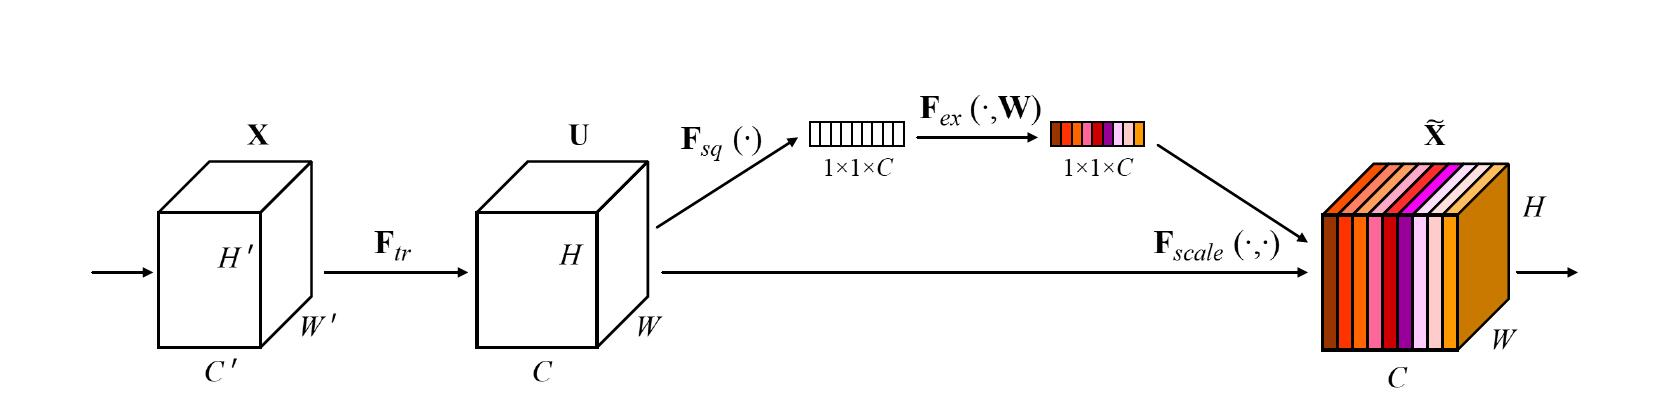
\includegraphics[width=14cm]{pic/chapter3/SENet.jpg}
  \caption{SENet 结构图\citing{hu2018squeeze}}
  \label{SENet}
\end{figure}

\subsection{空间注意力机制}
空间注意力机制是深度学习处理图像和空间数据中的注意力机制方法。其主要目的是通过对输入数据的不同空间位置引入不同的权重,赋予模型具备灵活关注对下游任务重要的区域的能力,提升模型对空间结构的感知能力。空间注意力模块(Spatial Attention Module, SAM)\citing{woo2018cbam}是一个经典的运用空间注意力机制的方法。如图\ref{SAM}所示,SAM的主要思想是首先利用最大池化层和平均池化层获得两个全局的特征图,然后通过拼接操作将两个特征图进行拼合,再利用一个$7\times 7$的卷积核将拼合的特征图转化成单通道的特征,最后使用sigmoid激活函数\citing{kyurkchiev2015sigmoid}得到空间注意力权值,并与原始输入进行相乘得到最终大小与输入相同的输出。空间注意力的计算公式如下式所示:
\begin{equation}
  \begin{aligned}
    \mathbf{M}_{\mathbf{s}}\left( \mathbf{F} \right) & =\sigma \left( f^{7\times 7}\left( \left[ AvgPool\left( \mathbf{F} \right) ;MaxPool\left( \mathbf{F} \right) \right] \right) \right)
    \\
                                                     & =\sigma \left( f^{7\times 7}\left( \mathbf{F}_{\mathbf{avg}}^{\mathbf{s}};\mathbf{F}_{\mathbf{max}}^{\mathbf{s}} \right) \right)
  \end{aligned}
\end{equation}

\begin{figure}[h]
  \centering
  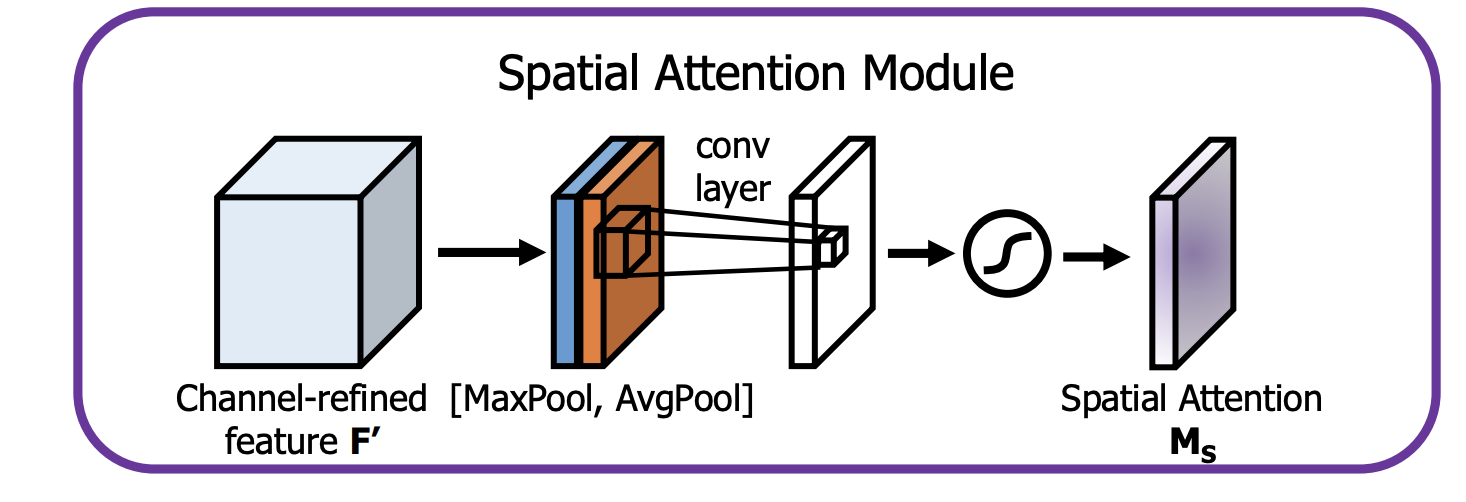
\includegraphics[width=14cm]{pic/chapter3/SAM.png}
  \caption{SAM 结构图\citing{woo2018cbam}}
  \label{SAM}
\end{figure}
\subsection{混合注意力机制}
混合注意力机制是综合多个注意力模块来处理数据的方法,通过对多个不同类型的注意力机制的融合,来增强深度网络模型对输入数据的建模能力,以更加灵活、全面地捕获输入数据的关键信息。卷积块注意力模块(Convolutional Block Attention Module, CBAM)\citing{woo2018cbam}是一个综合了通道和空间注意力机制的经典混合注意力方法。如图\ref{CBAM}所示,CBAM的主要网络架构有串联的通道注意力模块和空间注意力模块构成。通过依次使用通道和空间注意力模块,分别在通道和空间维度学习数据的关键信息,增强模型对输入数据的感知能力。其中,上一小节已经介绍了空间注意力模块的计算流程,而通道注意力机制的计算公式可以表示如下:
\begin{equation}
  \begin{aligned}
    \mathbf{M}_c\left( \mathbf{F} \right) & =\sigma \left( MLP\left( AvgPool\left( \mathbf{F} \right) \right) +MLP\left( MaxPool\left( \mathbf{F} \right) \right) \right)
    \\
                                          & =\sigma \left( \mathbf{W}_1\left( \mathbf{W}_0\left( \mathbf{F}_{avg}^{c} \right) \right) +\mathbf{W}_1\left( \mathbf{W}_0\left( \mathbf{F}_{max}^{c} \right) \right) \right)
  \end{aligned}
\end{equation}
其中,$\sigma$表示sigmoid函数,$W_0 \in \mathbb{R}^{C/r\times C}$、$W_1 \in \mathbb{R}^{C\times C/r}$均是多层感知机的权重参数。

因此,CBAM的计算流程可以表示为:
\begin{align}
  \mathbf{F}\prime=\mathbf{M}_{\mathbf{c}}\left( \mathbf{F} \right) \otimes \mathbf{F}
  \\
  \mathbf{F}''=\mathbf{M}_{\mathbf{S}}\left( \mathbf{F}\prime \right) \otimes \mathbf{F}\prime
\end{align}
其中,$\otimes$表示逐元素乘法。

\begin{figure}[h]
  \centering
  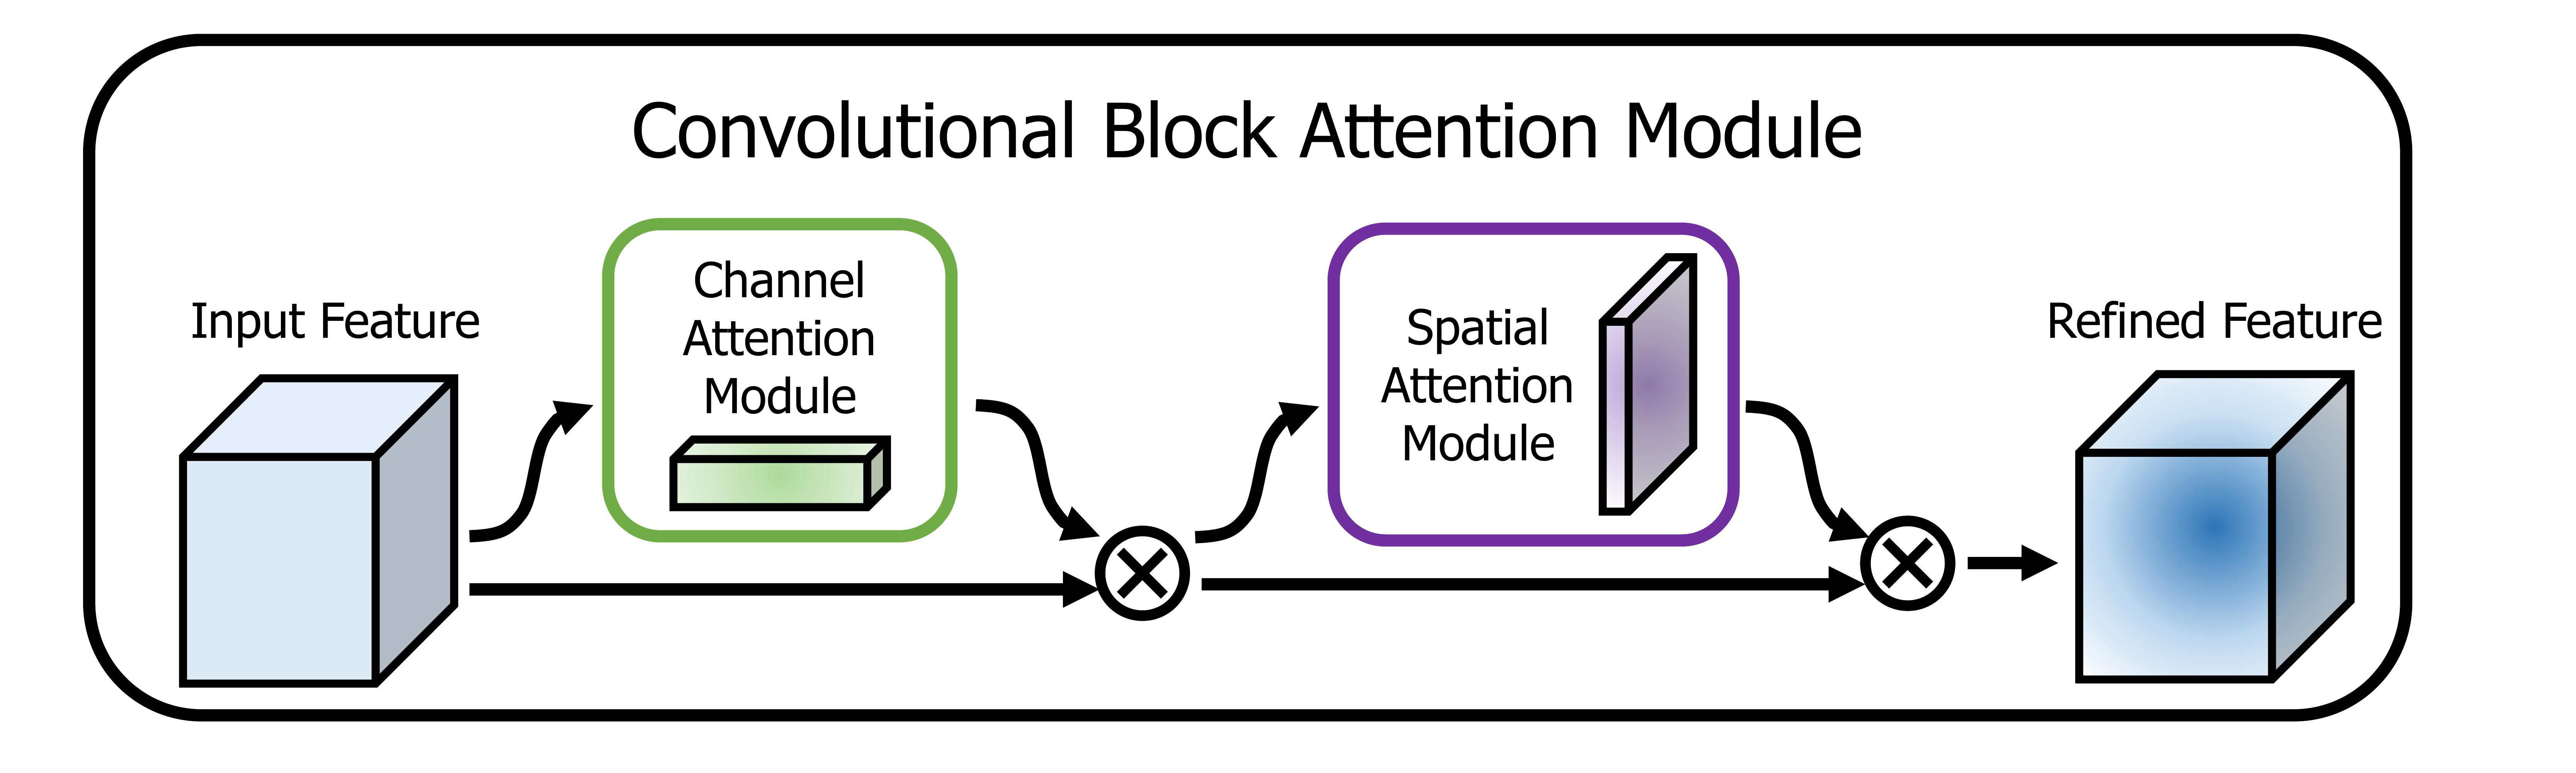
\includegraphics[width=14cm]{pic/chapter3/CBAM.jpg}
  \caption{CBAM 结构图\citing{woo2018cbam}}
  \label{CBAM}
\end{figure}

\section{基于双通道注意力的极化信息提取方法}
% 考虑到极化SAR图像原始数据可以由极化散射特征和极化目标分解特征进行表征,存在数据量大、信息复杂度高的问题,如果直接简单堆叠使用,甚至会导致模型性能下降。鉴于不同的地物目标之间散射特性存在差异,因此对极化SAR特征的重新标定校准是必不可少的,根据目标散射特性,自适应地增强有效特征,而抑制无效特征。为了高效地提取极化SAR数据中的有效信息,本章提出了一种基于双通道注意力的极化信息提取方法,旨在通过注意力机制来捕捉原始特征中的关键信息,充分考虑了不同极化特征之间的差异与联系,注重不同极化通道或空间中的关联性和权重分布,从而提高信息表征的准确性和效率。该方法可以作为一种即插即用的插件式网络结构,应用在后续的目标检测、地物分类任务中,为其提供更为可靠的基础极化信息表示。下面将详细介绍基于双通道注意力的极化信息提取方法的设计原理和实现步骤。

注意力机制方法目前已经广泛应用于图像处理领域,特别是计算机视觉和深度学习相关任务中,这些方法通过在网络结构中引入注意力机制方法对图像中特定区域的加权关注,使模型能够更加关注关键的信息,提升分类性能。然而,由于极化SAR图像的独特数据特征,包括复杂的多通道信息和多维度的散射机制,直接将通用的注意力机制方法应用于极化SAR图像处理任务可能效果不尽人意。为了更好的适应极化SAR图像处理的需求,本章基于极化相干信息与目标分解信息的差异性,提出了双通道注意力机制的网络结构,充分挖掘两类极化信息之间的差异性与关联性,为后续分类任务提供类内相聚、类间远离的良好的可分性极化特征,提升分类性能。


\subsection{双通道注意力极化信息提取网络框架}
% 图\ref{DPEN_framework}是基于双通道注意力的极化信息提取算法示意图。该极化信息提取模型由两个注意力通道构成:极化目标分解通道和极化散射特征通道。该方法的主要思路是:首先通过设计双注意力通道的结构,将目标分解特征和散射特征隔离输入,保证模型对不同层次的特征具有感知能力。然后,在每一个通道内,依次采用空间注意力和通道注意力来捕获输入特征的关键信息。为了强化极化信息的感知能力,设计了极化注意力调整模块,聚合不同层次的关键信息,对得到的注意力权重进行修正。其次,为了进一步提升模型的空间信息学习能力,引入跨空间学习模块,聚合不同尺寸的极化特征。最后,将两个通道的极化信息拼接形成最终的注意力增强的极化特征,用于下游分类任务的输入。

图\ref{DPEN_framework}是基于双通道注意力的极化信息提取算法示意图。该方法以提升极化信息可表达能力为目的,基于极化相干信息与极化目标分解信息之间的差异性,提出了双通道注意力机制的极化信息提取方法。该方法的主要思路是:首先,为了充分挖掘两类不同类型极化信息的关键信息,在两个独立的通道中分别利用注意力方法捕获输入特征的关键信息。其次,利用注意力联合调整模块,对两类信息的注意力权重进行动态调整,旨在结合两类极化信息的互补信息。然后,基于极化SAR的大空间尺寸特性,利用跨空间学习模块,聚合不同尺寸的极化特征。最后,将重新调整的极化特征进行拼接,形成注意力增强的极化特征。值的注意的是,本章提出的极化信息提取方法可以作为一个即插即用的插件式模块,应用到下游的目标检测、分类识别任务中。

\begin{figure}[h]
  \centering
  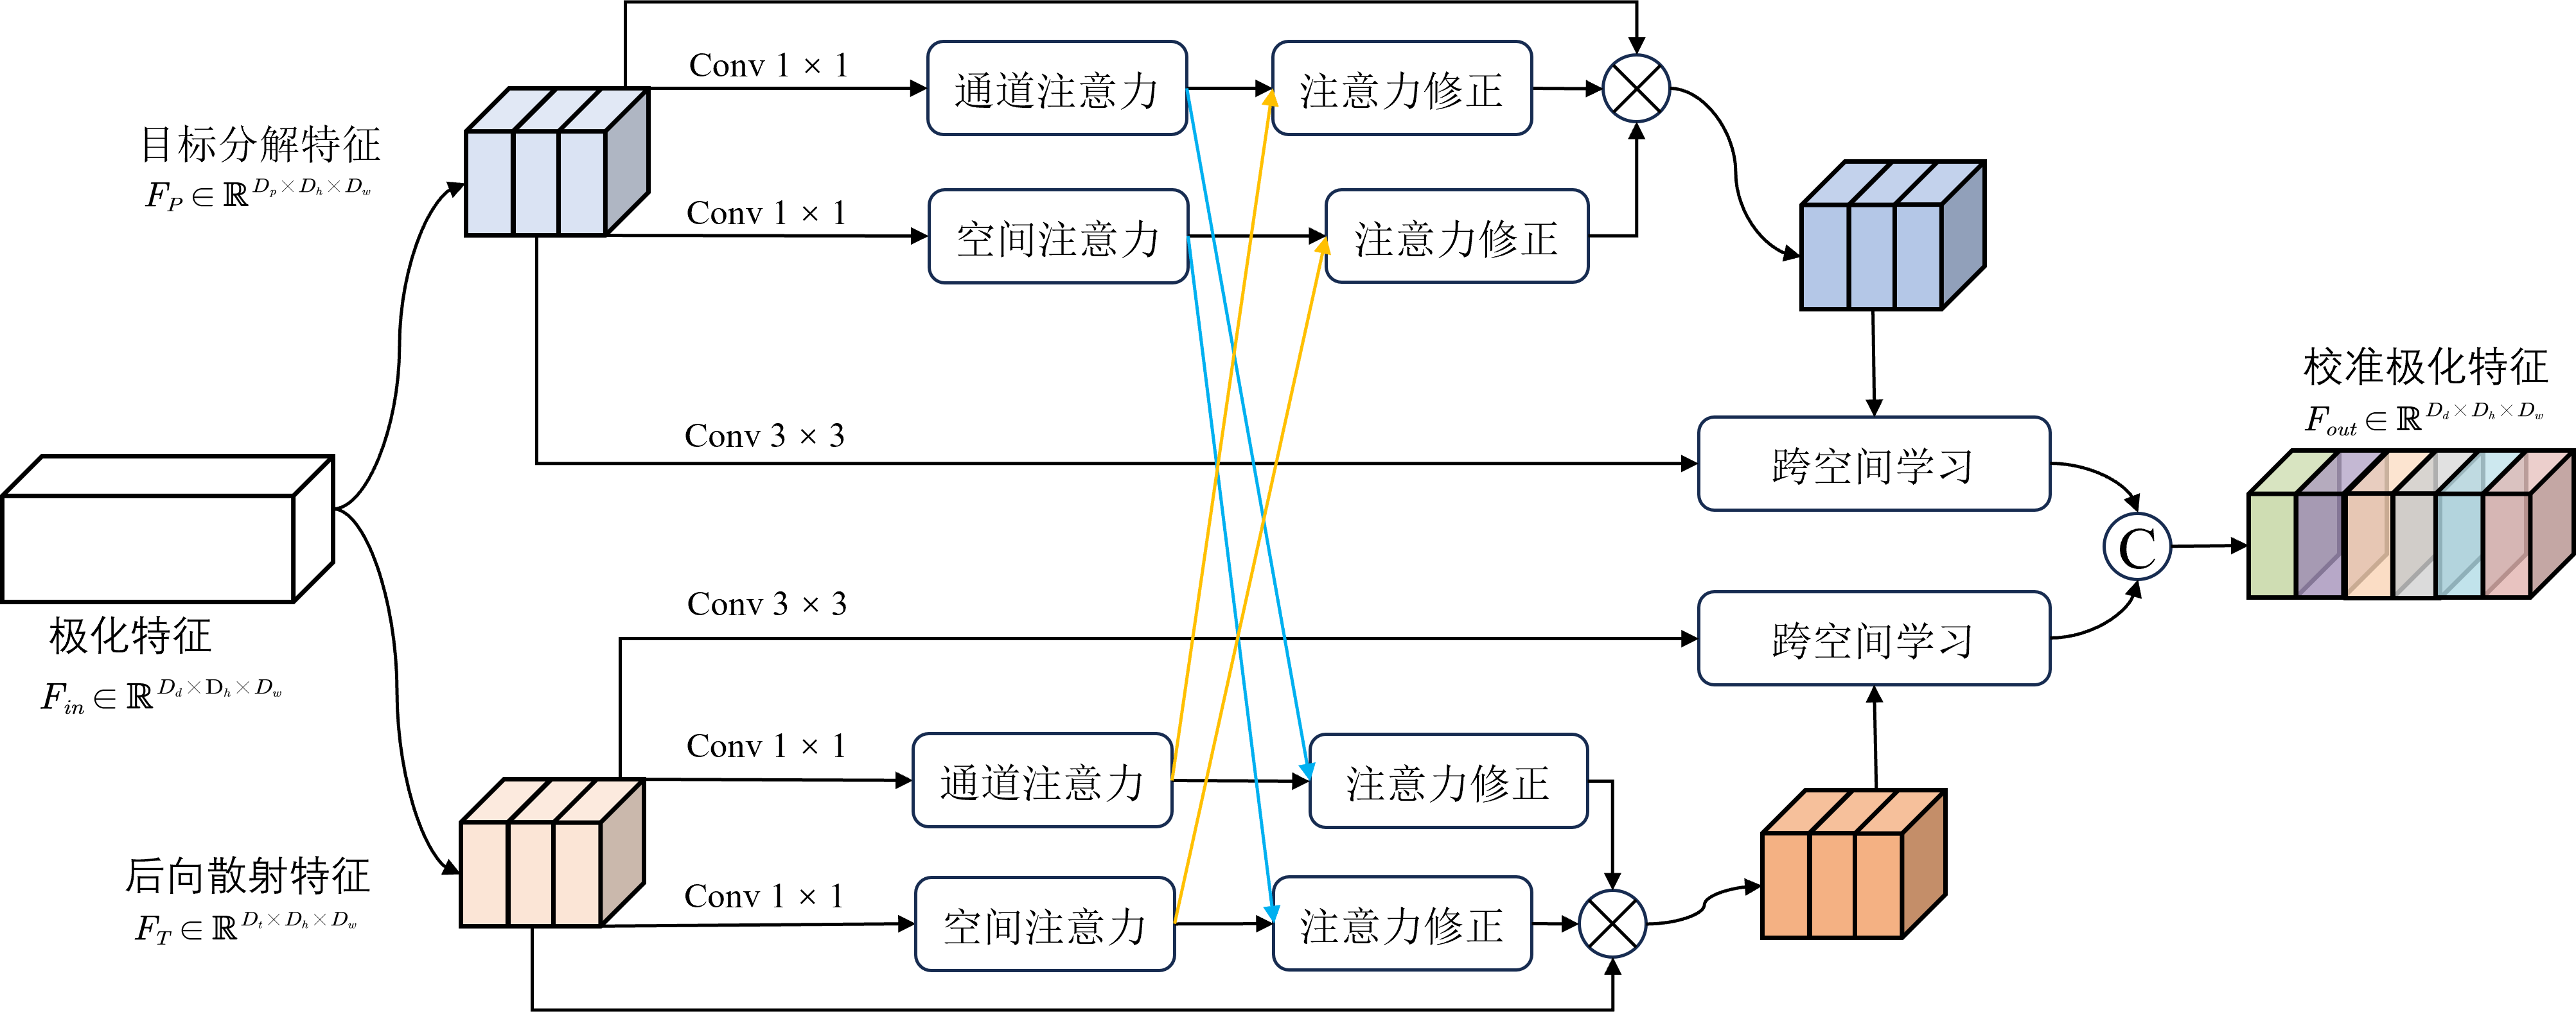
\includegraphics[width=14cm]{pic/chapter3/DPEN_framework.png}
  \caption{基于双通道注意力的极化信息提取算法示意图}
  \label{DPEN_framework}
\end{figure}

根据图\ref{DPEN_framework},网络输入为双独立通道形式,分别输入具有目标完备后向散射信息的极化相干矩阵和具有不同物理散射特性的极化目标分解特征。两路分支输入特征如下所示:

(1)通道1:后向散射特征

根据公式\ref{eq:T},极化相干矩阵$T$非主对角线元素均是复数,而主对角线元素均是实数,并且关于主对角线共轭对称。因此,可以使用矩阵的上三角6个元素代表极化相干矩阵,考虑到复数性质,使用一个包含9个元素的一维数组表示极化相干矩阵,具体如下式所示:
\begin{equation}
  \mathbf{V}=[T_{11}, T_{22}, \text{Re}(T_{33}), \text{Re}(T_{12}), \text{Re}(T_{13}), \text{Im}(T_{23}), \text{Im}(T_{33}), \text{Im}(T_{12}), \text{Im}(T_{13}), \text{Im}(T_{23})]
\end{equation}
其中,$\text{Re}$与$\text{Im}$分别表示取实部与取虚部运算。

$\mathbf{V}$包含了地物目标完备的后向散射信息,将$\mathbf{V}$作为通道1的输入。

(2)通道2:目标分解特征

不同的极化目标分解特征从不同的物理层面反映了目标的散射特性,通道2选择多种经典的极化目标分解特征作为输入,分别为Pauli分解、Cloude分解、Freeman分解、Krogager分解、Huynen分解共计32维目标分解参数。具体特征参数如表\ref{tab:decomposition_features}所示。

\begin{table}[ht!]
  \caption{通道2使用的极化目标分解特征参数表}
  \label{tab:decomposition_features}
  \centering
  \begin{tabular}{cccc}
    \toprule[1.5bp]
    分解方法                     & 特征参数                                                             & 物理意义               & 特征维数 \\
    \midrule[0.75bp]
    Pauli                    & $\left| a \right|^2,\left| b \right|^2,\left| c \right|^2$
                             & 奇次、偶次、二面角散射                                                      & 3                         \\
    \multirow{2}{*}{Cloude}  & $H,\alpha,A$                                                     & 散射熵、平均散射角、反熵       & 3    \\
                             & $\lambda_1,\lambda_2,\lambda_3$                                  & 极化相干矩阵特征值          & 3    \\
    \multirow{2}{*}{Freeman} & $P_s,P_d,P_v,P_r$                                                & 表面散射、体散射、二次散射、同极化比 & 4    \\
                             & $f_s,f_d,f_v$                                                    & Freeman系数          & 3    \\
    Krogager                 & $\left| k_s \right|^2,\left| k_d \right|^2,\left| k_h \right|^2$ & 球、双平面、螺旋散射能量       & 4    \\
    \multirow{3}{*}{Huynen}  & $A_0,B_0+B,B_0-B$                                                & 对称、非对称、不规则性信息      & 3    \\
                             & $C,D,E$                                                          & 线性、弯曲、扭转性信息        & 3    \\
                             & $F,G,H$                                                          & 螺旋、沾合、方向信息         & 3    \\
    Van Zyl                  & $f_v,f_d,f_s$                                                    & 体散射、二次散射、表面散射系数    & 3    \\
    \bottomrule[1.5bp]
  \end{tabular}
\end{table}

方法流程叙述方法流程叙述方法流程叙述方法流程叙述方法流程叙述方法流程叙述方法流程叙述方法流程叙述方法流程叙述方法流程叙述方法流程叙述方法流程叙述

\subsection{空间和通道注意力模块}
% 引入空间和通道注意力模块,旨在提升对应层次特征通道中特征的可鉴别特性。通过通道注意力自适应地校准每个通道特征图的权重、空间注意力来捕捉像素级的空间信息,在重要的特征上得到增强,而在不相关的特征上权重较小。图\ref{scSE}为scSE的结构图,包含了两个并行的模块,分别是用于提取通道注意力的cSE(channel Squeeze Excitation, cSE)和用于提取空间注意力的sSE(spatial Squeeze Excitation, sSE),输入的特征图$F$经过这两个模块的重新校准,输出校准后的特征图$F_{sSE}$和$F_{cSE}$。基于以上的校准模型,能够学习到空间、通道两种维度上更加有意义的信息。

% 如图\ref{scSE}所示,相比于SE模块的全连接层,sSE空间注意力模块采用卷积操作来获取全局信息,从而赋予其更多的非线性捕捉能力,更好的拟合不同空间位置之间的复杂相关性,显著减少参数量和计算量。如图\ref{scSE}所示,sSE模块首先对每个通道素具进行压缩,利用$1\times 1 \times 1$卷积,将输入的特征图$F$的特征维度从$H \times W \times C$压缩为$H \times W \times 1$,然后利用Sigmoid激活函数得到空间注意力系数图。系数图中的每一个像素点代表了所有通道的特征图在该空间位置信息的重要程度。基于空间注意力系数图能够使模型更加关注与任务相关的空间位置信息,而抑制不相关的位置信息。

% cSE模块首先对输入的特征图在特征通道上进行压缩,通过全局平均池化的方式,将特征维度为$H \times W \times C$的输入特征压缩为$1 \times 1 \times C$维度。全局平均池化操作对输入特征图的空间依赖性进行拆解,并通过逐个学习每个通道生成反映各个通道重要性的特征图。随后,这些特征图经过两个卷积层进行信息处理,最终被转换为$C$维向量。经过Sigmoid激活函数处理后,得到相应的通道注意力权重系数,该系数用于表示不同通道特征图的重要性。利用通道注意力权重系数,动态调整每个通道的重要程度,以更加精准地捕捉有助于任务的特征信息,提升模型对关键特征的敏感性。


注意力方法通过强调或抑制输入特征中的不同部分,在深度学习领域,被广泛应用到各种任务中。本文通过引入空间和通道注意力方法,旨在对输入的极化信息动态调整关注度,提升模型对关键信息的感知能力。图\ref{fig:spatial}为本方法中的空间注意力模块网络结构。空间注意力方法采用卷积操作来获取全局信息,从而赋予其更多的非线性捕捉能力,更好的拟合不同空间位置之间的复杂相关性,显著减少参数量和计算量。计算公式如下所示:
\begin{equation}
  A_s=\sigma(f^{7\times 7}(AvgPool(S);\Gamma(MaxPool(S))))
\end{equation}
其中,$f^{7\times 7}$表示卷积核大小为$7\times 7$的卷积操作;$\sigma$表示Sigmoid激活函数。空间注意力通过最大池化和平均池化两个池化操作得到大小为$2\times H \times W$的特征图,最大池化从图像中提取强的局部信息,平均池化提取全局平均统计特征。对特征图采用卷积运算,转换为$1\times H\times W$的单一通道特征,再利用Sigmoid激活函数将通道特征图转为对应的空间注意力图$A_s$,最后计算注意力图$A_s$与原始输入特征的乘积得到空间注意力信息。计算公式如下:
\begin{equation}
  S_S=A_S \otimes S
\end{equation}
其中,$\otimes$ 表示逐元素乘积。通过空间注意力方法,在空间维度进行有效信息激发而抑制无效信息,得到空间注意力图校准的极化特征$S_S$。

\begin{figure}[ht!]
  \centering
  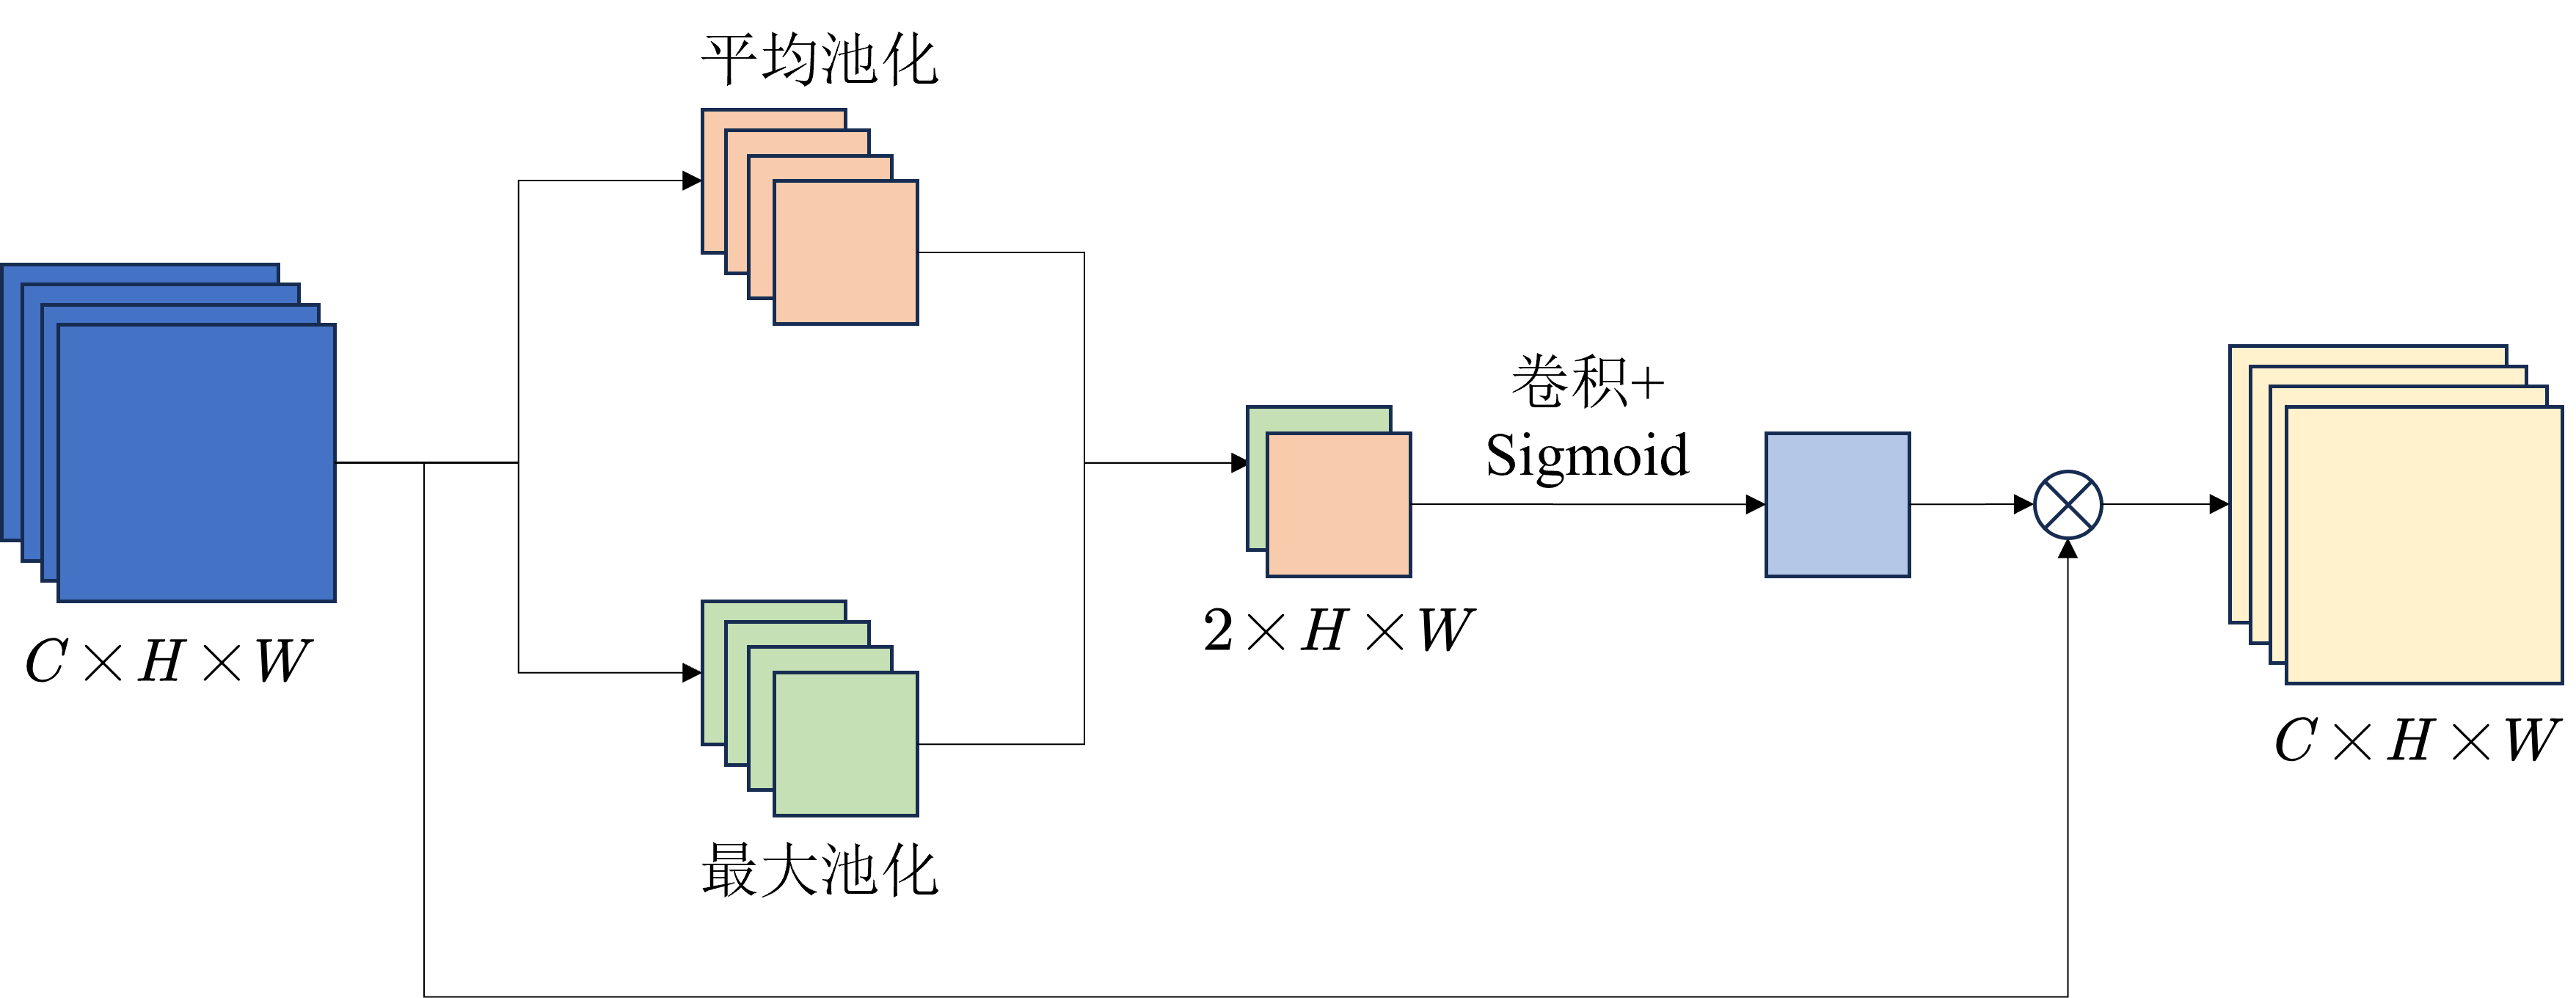
\includegraphics[width=14cm]{pic/chapter3/Spatial.png}
  \caption{空间注意力模块结构}
  \label{fig:spatial}
\end{figure}

相比于空间注意力方法使用卷积层层与激活函数的注意力提取方法,通道注意力方法通过全连接和加和操作,完成对通道维度信息的提取。全局最大池化与平均池化操作对输入特征图的空间依赖性进行拆解,并通过逐个学习每个通道生成反映各个通道重要性的特征图。随后,将得到的两个$C\times 1 \times 1$的特征图进行拼接后使用全连接和加和运算后,再使用Sigmoid激活函数,形成成一维的通道注意力图,用于表示不同通道特征图的重要性。计算如下式所示:
\begin{equation}
  A_C=\sigma(\Gamma(AvgPool(S))+\Gamma(MaxPool(S)))
\end{equation}
其中,$\sigma$表示Sigmoid激活函数;$\Gamma$表示两层神经网络。将通道注意力图与输入极化特征相乘,得到通道注意力图校准的极化特征。计算公式如下:
\begin{equation}
  S_C=A_C \otimes S
\end{equation}
其中,$\otimes$表示逐元素乘法。

\begin{figure}[ht!]
  \centering
  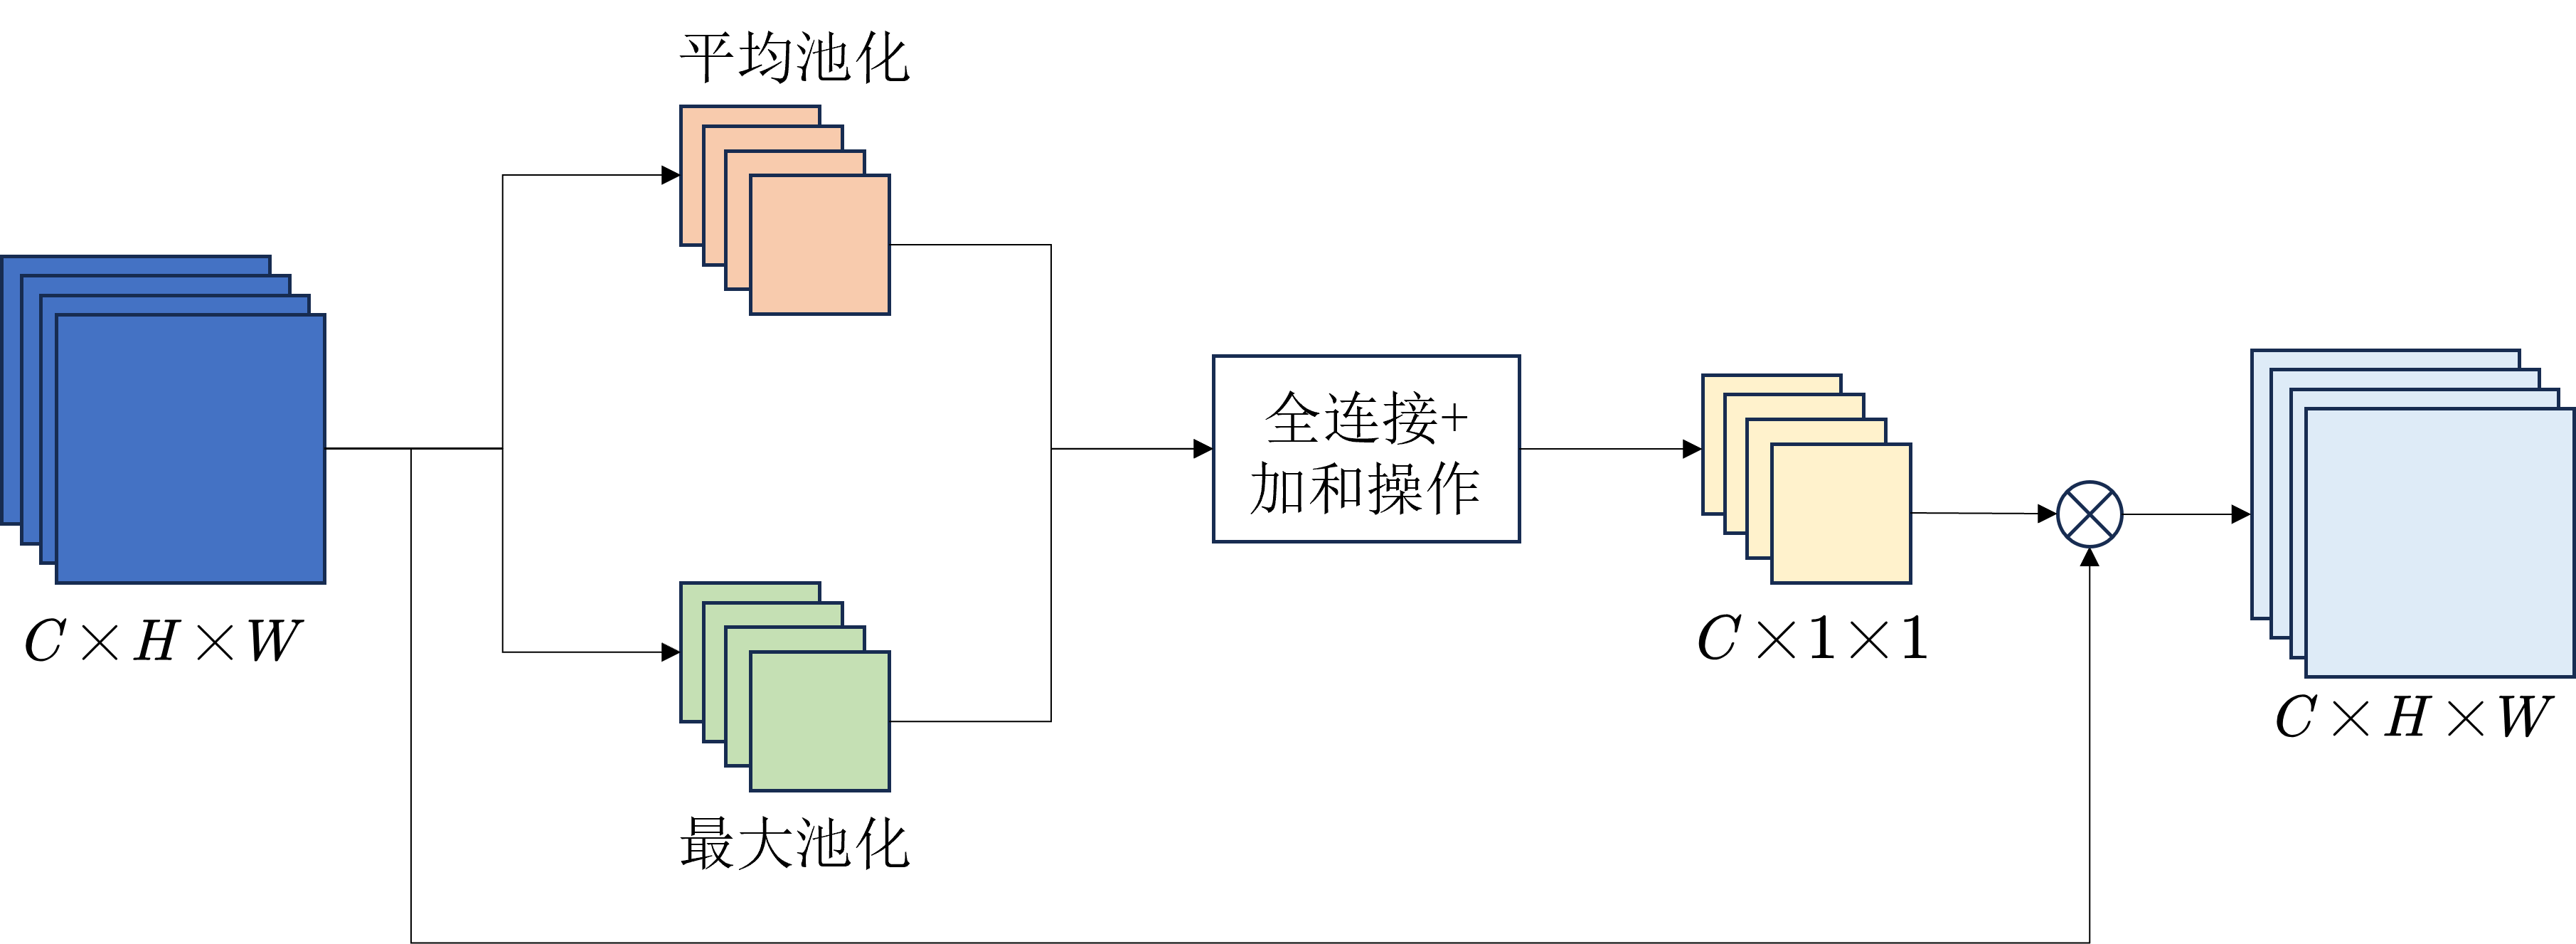
\includegraphics[width=14cm]{pic/chapter3/Channel.png}
  \caption{通道注意力模块结构}
  \label{fig:channel}
\end{figure}


\subsection{极化注意力修正模块}
基于双通道注意力架构对极化SAR输入特征提取空间、通道注意力特征图,对于同一类型目标,校准后的两种类型极化信息存在一致性与互补性。为了保持特征一致性和挖掘极化互补信息,图\ref{DPEN_WFM}展示的极化注意力修正模块,以极化信息一致性为引导,对输入的极化特征进行动态调整。极化注意力修正模块利用输入的一路极化特征作为主要引导,对另外一路特征进行修正。其中主要包含卷积与残差运算,计算公式如下所示:
\begin{gather}
  S_{1}^{\prime}=f^{1\times 1}\left( f^{1\times 1}\left( S_1 \right) \right) \times f^{1\times 1}\left( f^{1\times 1}\left( S_1 \right) \right)
  \\
  S_{2}^{\prime}=f^{1\times 1}\left( S_2 \right)
  \\
  S_{out}=S_1+\left( S_{1}^{\prime}\times S_{2}^{\prime} \right)
\end{gather}

\begin{figure}[h]
  \centering
  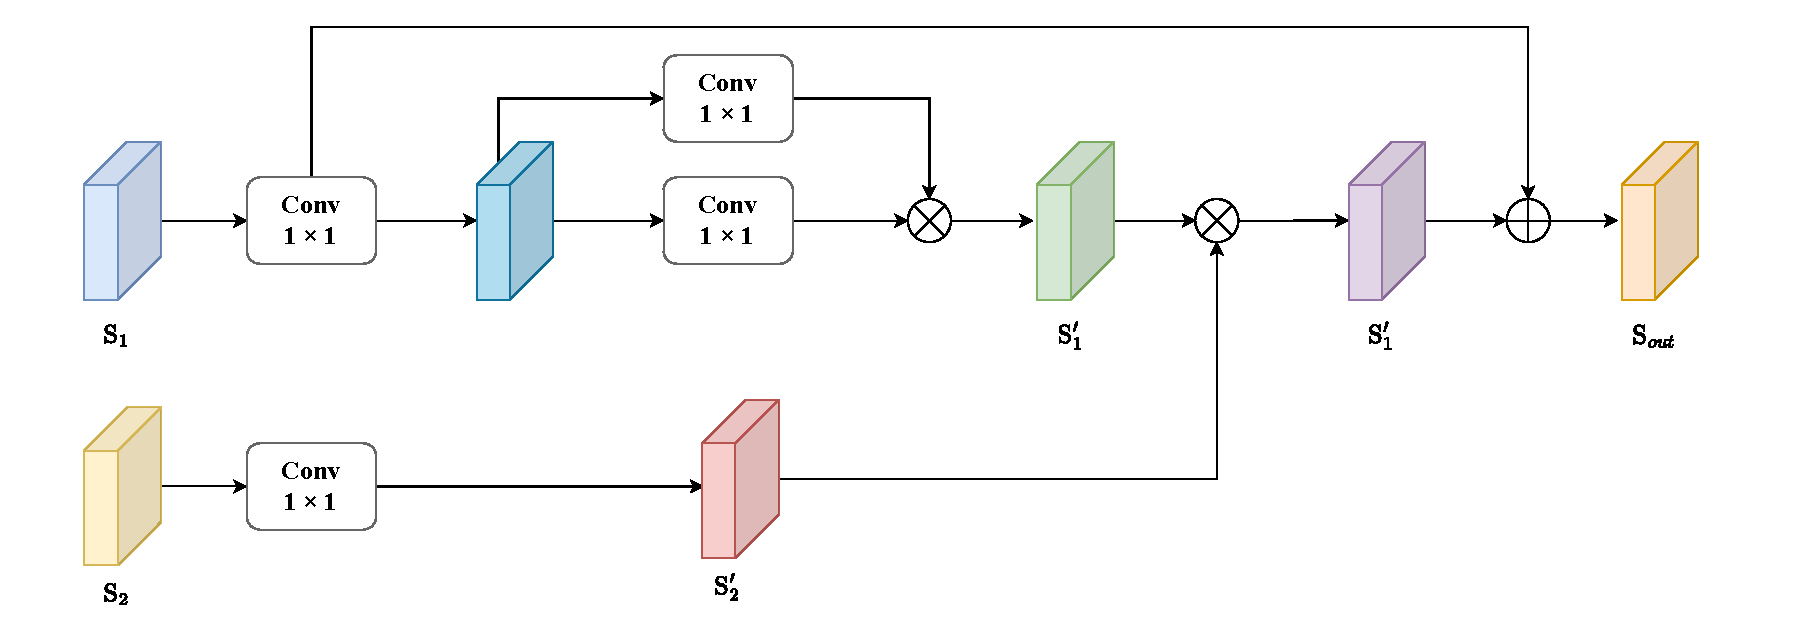
\includegraphics[width=14cm]{pic/chapter3/极化注意力修正.pdf}
  \caption{极化注意力修正模块结构示意图}
  \label{DPEN_WFM}
\end{figure}


\subsection{跨空间学习模块}
跨空间学习模块的网络结构如图\ref{DPEN_CSL}所示。跨空间学习模块提供了一种不同空间维度方向的极化信息聚合方法,来实现多尺度下的极化特征聚合。引入两个分支的张量,分别是$1\times 1$分支的输出和$3 \times 3$分支的输出。随后利用二维全局平均池化对$1\times 1$分支的输出中的全局极化空间信息进行编码,用于编码全局信息和建模远程依赖关系。二维全局池化操作可以表示为:
\begin{equation}
  z_c=\frac{1}{H\times W}\sum_{j}^{H}\sum_{i}^{W}x_c(i,j)
\end{equation}

在以上二维全局平均池化的输出处采用二维高斯映射的自然非线性函数Softmax来拟合线性变换,进而提升计算效率。通过将上述并行处理的输出与矩阵点积运算相乘,得出了第一个空间注意力图。同样利用二维全局平均池化在$3\times 3$分支编码全局空间信息,将每组内的输出特征映射计算为生成的两个空间权重值的集合,然后使用Sigmoid函数映射成空间位置对应的权重关系。通过捕获像素级的成对关系,突出显示所有像素的全局上下文信息。计算公式如下:
\begin{gather}
  S_1=f^{1\times 1}\left( S \right) \times \mathrm{AvgPool}\left( f^{3\times 3}\left( S \right) \right)
  \\
  S_2=f^{3\times 3}\left( S \right) \times \mathrm{AvgPool}\left( f^{1\times 1}\left( S \right) \right)
  \\
  S^{\prime}=\sigma \left( S_1+S_2 \right)
\end{gather}
其中,$\sigma$表示sigmoid函数。

\begin{figure}[ht!]
  \centering
  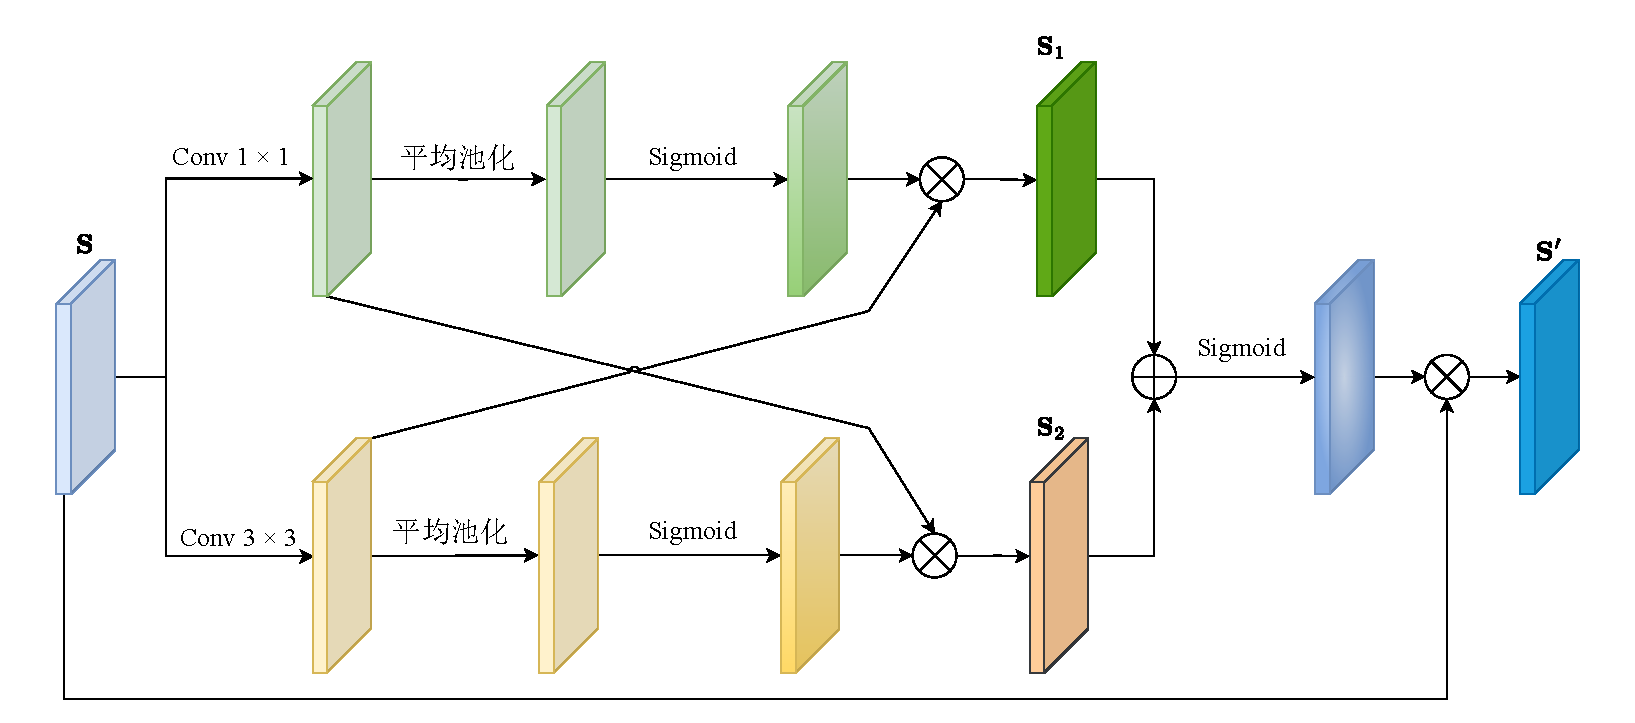
\includegraphics[width=14cm]{pic/chapter3/跨空间学习.pdf}
  \caption{CSL 结构图}
  \label{DPEN_CSL}
\end{figure}


\section{实验结果与分析}
\subsection{实验模型介绍}
本章实验所使用的计算环境为一台CPU为Intel Core i7-8700K和配备了NVIDIA GPU(GeForce RTX 3090, 24G)的计算机设备。操作系统采用Ubuntu 20.04 LTS。深度学习框架选择PyTorch,版本为1.9.0,同时依赖CUDA深度神经网络库(cuDNN)版本8.0.5。在科学计算方面,实验使用NumPy库,版本为1.19.5。

学习率作为深度学习模型训练的关键参数之一,其值的选择对于模型的收敛速度至关重要。在训练过程中,如果学习率设置的过大或者过小,均会可能给模型的分类准确度产生负面影响。通常情况下,在模型的训练初始阶段,采用较大的学习率能够使模型快速收敛到最优点附近。随着训练的执行,逐渐减小学习率,以更加精确地接近最优点。在本章所采用的模型中,初始学习率为$3\times 10^{-4}$,在训练至第30至60个epoch期间,学习率经过衰减变为原值的0.1倍。这里的epoch表示训练集中素有样本完成一次正向传递和反向传播的过程,本章中模型训练的epoch设置为100。Batch size表示每次训练中选择的样本数量,其值的大小会影响网络的优化速度和执行效率。在本章模型中,batch size被设置为64。

% 实验中,使用两组真实极化SAR数据集分别是荷兰Flevoland区域和德国Oberpfaffenhofen地区数据来验证本章方法的有效性,并利用常规的性能指标总体分类准确率(OA)、各个类别分类准确率和Kappa系数对分类结果进行数值量化。同时对分类的可视化结果进行视觉评估。在给定的极化SAR标准数据集中,一部分像素是没有标签的,所以在计算分类准确率的时候只统计数据集中那些有标签的样本被正确分类的百分比,并认为该指标可以表征数据集中整体的分类性能。

本章基于双通道注意力的极化信息提取器(Dual-attention Polarization information extractor,简记为DP),可以作为插件式组件应用到下游的分类任务中。为了验证本章方法的有效性与优越性,基于DP构建端到端的极化SAR图像特征提取与分类方法(记为DP-CNN),网络结构如图\ref{fig:DPCNN}所示,分为极化信息提取和分类器两个部分。从输入的高维原始极化特征出发,利用DP模块可以获得全局信息并且嵌入到分类器中。原始极化特征中有价值的信息被激发,而没有价值的信息被抑制。当具备了重新校正的极化特征之后,基于深度神经网络实现极化SAR图像的分类。在本节的实验方法中,使用一个类似vgg的卷积架构来实现特征提取与分类流程。具体而言,该卷积架构包括三个带有ReLu激活函数的$3\times 3$卷积层、三层最大池化函数、两层全连接网络以及一层SoftMax激活层构成。

\begin{figure}[ht!]
  \centering
  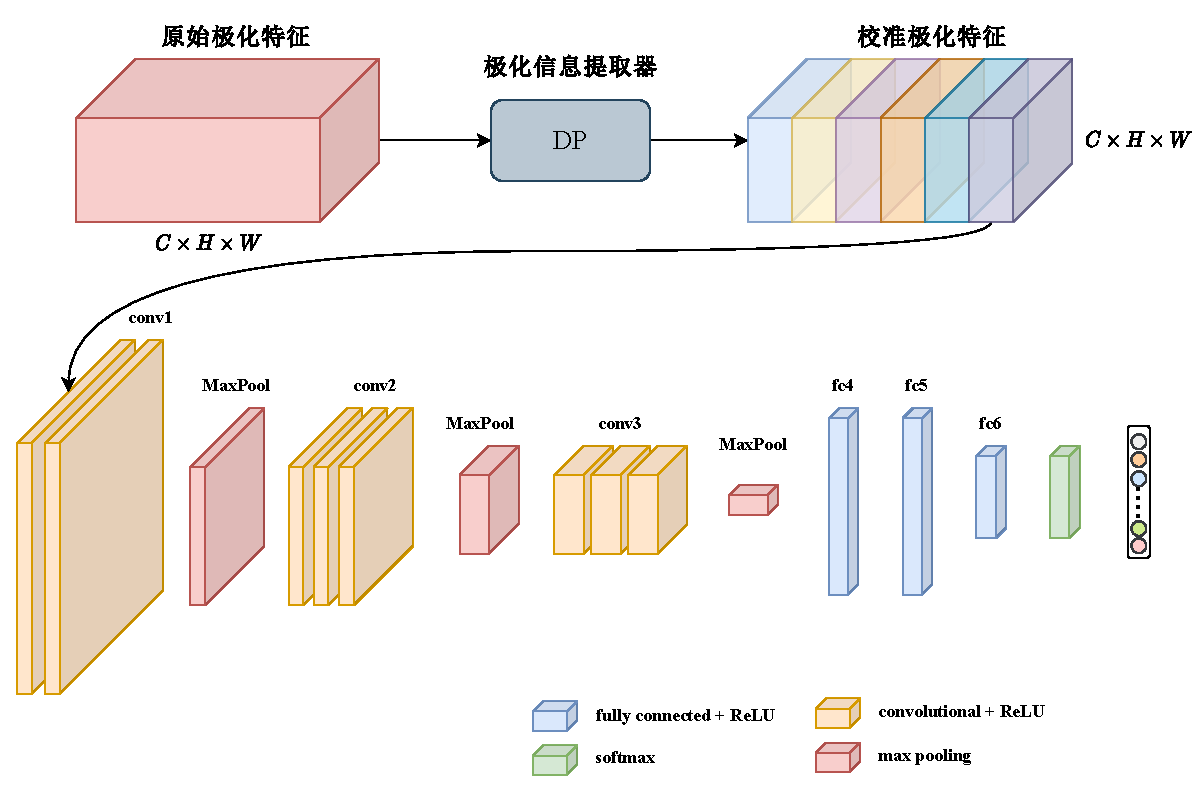
\includegraphics[width=14cm]{pic/chapter3/DPCNN.pdf}
  \caption{DP-CNN网络结构示意图}
  \label{fig:DPCNN}
\end{figure}


以交叉熵损失函数\citing{}为目标,通过反向传播算法训练模型参数。交叉熵损失时分类问题中最常用的损失函数之一,衡量了分类模型的预测值与真实标签之间的差异性,是一种用于优化分类模型的目标函数。

综上所述,本章的DP-CNN方法将输入的原始极化特征$x$映射为预测概率$p\in \mathbb{R}^{C}$,其中,$C$表示类别的个数。$x$对应的中心像素预测标签可以通过选择概率最高的类别,即向量$p$的最大值索引来预测。其计算公式如下:
\begin{equation}
  H(p,q)=\sum_{i=1}^{n}p(x_i)log(q(x_i))
\end{equation}
其中,$p(x)$表示真实值分布概率,$q(x)$表示模型预测分布概率。交叉熵值的变化与模型的训练效果密切相关,优越的训练效果会让预测概率分布逐渐趋近于真实值概率分布,相应的交叉熵值会逐渐减少。Sigmoid和Softmax损失函数是两个被广泛应用的交叉熵损失函数。Sigmoid损失函数主要应用于多标签分类任务,其中分类目标可以同时拥有多个标签。这一损失函数模拟了模型对多个独立事件的概率预测,每个事件的概率值落在$[0,1]$区间内。Softmax损失函数被广泛应用在多类别分类任务重,其中每个样本仅能关联一个类别。Softmax函数将预测模型的原始输出转化为表示类别概率的分布,确保所有类别的概率之和为1,并且模型的输出是互斥的。本章的极化SAR图像目标分类任务属于多分类语义分割任务,每个像素都有唯一的正确类别。因此选择多分类交叉熵损失函数,即Softmax损失函数作为模型的损失函数,为模型训练提供有力的优化目标。

为了对本章提出的极化信息提取方法进行全面地评估和对比,选择了多种替代方案进行比较,主要涉及两个方面的变化:一方面是对特征输入的处理改变,另一方面是对极化信息提取模块的替代策略。首先在特征输入方面,验证了不同极化特征表示对目标分类任务的影响。利用本章提出的基于双通道注意力的极化信息提取方法结合CNN分类模块进行分类、仅使用极化相干矩阵中的元素结合CNN分类方法(记为CNN-T)、仅使用极化目标分解特征结合CNN分类方法(记为CNN-P)、基于散射特征和分解特征简单叠加结合CNN的分类方法(记为CNN-F)作为不同的对比方法,验证本章方法在极化特征表示方面的有效性。其次是在极化信息提取模块层面进行替换,利用基于压缩和激励网络结合CNN分类方法(记为CNN-SE)和基于空间通道注意力结合CNN分类方法(记为CNN-CBAM)作为不同的对比方法,验证本章方法在极化特征表示方面的优越性。在每组实验中,从每个类别选择1\%的带标签像素,以这些带标签像素为中心,在其周围利用$15 \times 15$的窗口截取图像,形成训练集的样本表示。

\subsection{精度评价方法}
精度评价是对实际数据和模型分类结果进行比较的重要步骤,旨在确定分类模型的准确性,是衡量分类结果可靠性的关键指标。混淆矩阵(Confusion Matrix)通常作为遥感图像分类准确性能的评判指标,并且可以通过混淆矩阵计算得到多种常用的评价参数指标,例如总体分类准确率(Overall Accuracy, OA)、各个类别分类准确率、各个类别平均分类准确率(Average Accuracy, AA)、Kappa系数等。

混淆矩阵是一个$n \times n$的矩阵,其中$n$表示数据集的类别数量。混淆矩阵的行表示实际类别,列表示预测类别。其中,每个元素$(i, j)$表示实际属于类别$i$的样本被预测为类别$j$的数量。混淆矩阵主对角线元素表示被正确分类的样本,非主对角线表示分类错误的样本。

在极化SAR图像分类结果精度评价中,可以基于混淆矩阵定义以下指标:

1.总体分类准确率(OA):
\begin{equation}
  OA=\frac{\mbox{主对角线元素之和}}{\mbox{混淆矩阵所有元素之和}}
\end{equation}

2.生产者精度:
\begin{equation}
  \mbox{生产者精度}=\frac{\mbox{类别对应的主对角线元素}}{\mbox{类别所在列总和}}
\end{equation}

3.使用者精度。
\begin{equation}
  \mbox{使用者精度}=\frac{\mbox{类别对应的主对角线元素}}{\mbox{类别所在行总和}}
\end{equation}

4.错分误差。
错分误差是指被分类模型错误地划分为用户感兴趣的类别,实际上属于另一类别的样本数量,反映了模型在预测时产生的误报情况。
\begin{equation}
  \mbox{错分误差}=1-\mbox{使用者精度}
\end{equation}

5.漏分误差。
漏分误差是指本应该属于地表真实分类的样本,但是由于模型未能正确分类而被判为其他类别的数量,反映了模型在预测时产生的漏报情况。
\begin{equation}
  \mbox{漏分误差}=1-\mbox{生产者精度}
\end{equation}

6.Kappa系数
Kappa系数是一种通过多元统计方法来评价分类精度的指标,旨在量化分类模型的性能相对于完全随机分类的优越性。该系数通过考察混淆矩阵的对角线元素以及总体分布情况,提供了对分类结果误差的全局度量。具体计算公式如下:
\begin{equation}
  K=\frac{p_0-p_e}{1-p_e}
\end{equation}
其中,$p_0$表示总体分类精度,由主对角线元素之和除以所有样本数量计算得到;$p_e$表示某一个类别地表真实样本总数与该类中被分类样本总数之积对所有类别求和除以总样本数的平方。将混淆矩阵中的具体元素带入上式,可以得到:
\begin{equation}
  K=\frac{N\sum_{i=1}^{r}{{x_i}_i}-\sum_{i=1}^{r}{\left( {x_i}_+x_{+i} \right)}}{N^2-\sum_{i=1}^{r}{\left( {x_i}_+x_{+i} \right)}}
\end{equation}

Kappa系数的大小可以用来表示分类的精度性能,表\ref{kappa}描述了Kappa系数与模型的分类精度的映射关系。
\begin{table}[ht]
  \caption{Kappa统计值与分类精度映射关系}
  \begin{tabular}{cc}
    \toprule[1.5bp]
    Kappa系数 & 分类精度 \\
    \midrule[0.75bp]
    <0      & 较差   \\
    0-0.2   & 差    \\
    0.2-0.4 & 正常   \\
    0.4-0.6 & 好    \\
    0.6-0.8 & 较好   \\
    0.8-1   & 非常好  \\
    \bottomrule[1.5bp]
  \end{tabular}
  \label{kappa}
\end{table}

\subsection{AIRSAR Flevoland数据实验}
实验数据集选择NASA/JPL于1989年在Flevoland区域采集得到的全极化数据。该数据集是荷兰的一个农业区域遥感数据,作为基准数据集广泛应用于极化SAR土地覆盖目标分类研究中。该图像大小为$1024 \times 750$ 像素,共有15种农作物类别,包括茎豆、豌豆、森林、苜蓿、小麦、甜菜、土豆、裸土、草、油菜籽、大麦、水和少量建筑物。各个农作物目标类别之间的差异较小,相似性较强,因此分类难度较大,容易出现错分漏分的现象。图\ref{flevoland_pauli}和图\ref{flevoland_gt}分别展示了AIRSAR Flevoland数据集的Pauli分解伪彩图像以及对应的地面真值标签图像。表\ref{flevoland_smaple}展示了该数据集中每个类别带标签的样本数量。
\begin{figure}[ht]
  \subfloat[]{
    \label{flevoland_pauli}
    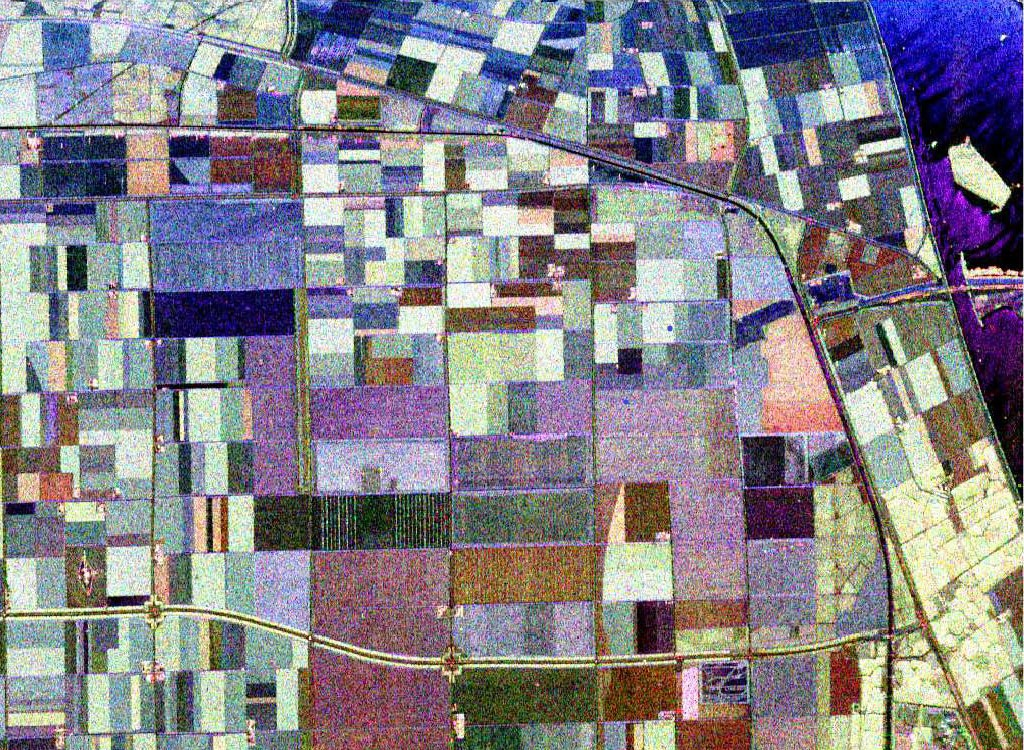
\includegraphics[width=7.04cm]{pic/chapter3/fle/pauli.png}
  }
  \subfloat[]{
    \label{flevoland_gt}
    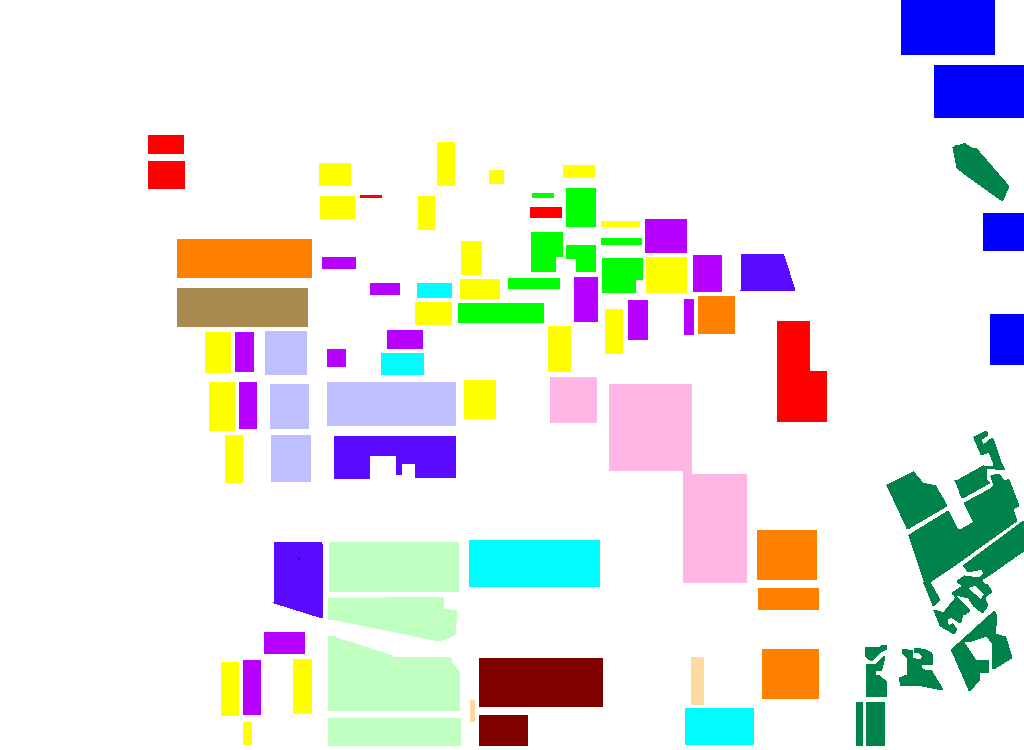
\includegraphics[width=7.04cm]{pic/chapter3/fle/gt.png}
  }

  \subfloat[]{
    \label{pice}
    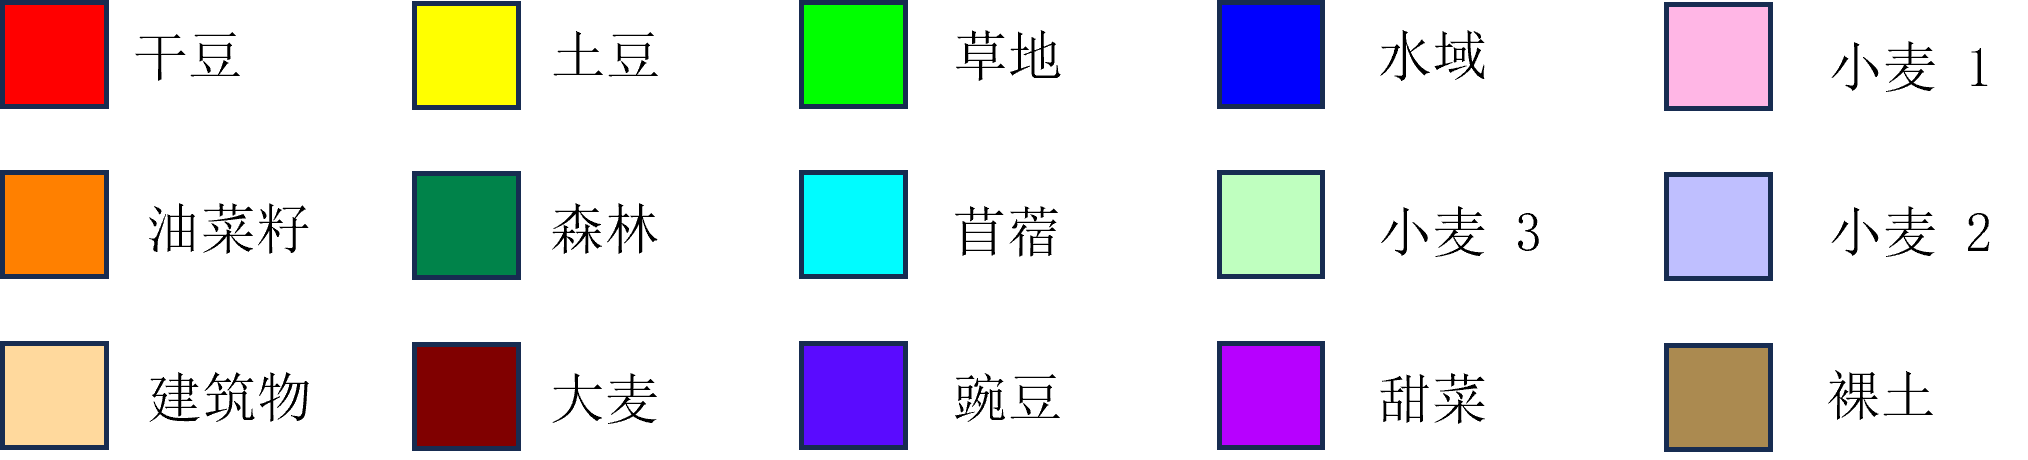
\includegraphics[width=9.04cm]{pic/chapter3/fle/label.png}
  }
  \caption{Flevoland地区实验数据集。(a)Pauli分解伪彩色图像;(b)实验数据地面真值;(c)颜色与类别对应关系}
  \label{fig2}
\end{figure}

\begin{table}[h]
  \caption{Felvoand地区实验数据集有标签样本数量}
  \begin{tabular}{|c|c|c|c|c|c|c|c|c|}
    \hline 类别 & 干豆   & 大麦    & 裸土    & 土豆    & 甜菜    & 小麦 1  & 豌豆    & 苜蓿
    \\
    \hline 数目 & 6338 & 7595  & 5109  & 16156 & 10033 & 11159 & 9582  & 10181 \\
    \hline 类别 & 草地   & 小麦 2  & 油菜籽   & 小麦 3  & 建筑物   & 森林    & 水域    &       \\
    \hline 数目 & 7058 & 16386 & 13863 & 22241 & 735   & 18044 & 13232 &       \\
    \hline
  \end{tabular}
  \label{flevoland_smaple}
\end{table}

图\ref{fig:fle_res}展示了各个对比方法的可视化分类结果。根据图\ref{fig:fle_T},仅使用散射特征的分类方法,在大麦、草地和小麦区域都有较多的错分样本,这是因为只使用了散射特征而忽略了目标分解特征,没有全面综合利用所有的极化信息导致的。图\ref{fig:fle_P}展示了仅使用目标分解特征的分类结果,在甜菜、小麦区域也存在大量的错分样本,这可能是由于没有综合使用极化信息导致的,相干矩阵代表的散射特征是极化SAR中最基本、重要的特征。图\ref{fig:fle_F}展示的简单叠加散射特征与目标分解特征的分类结果,该方法的分类结果要优于前面两种方法,类间错分孤立点相对减少,具有更少的错分样本,这反映了综合利用极化信息对目标分类具有一定的优势。图\ref{fig:fle_SE}与图\ref{fig:fle:CBAM}展示了使用经典注意力方法的分类结果图,相比于直接叠加特征,并没有带来明显的分类性能提升,少量的错分孤立点依然存在。图\ref{fig:fle_DP}展示了基于双通道注意力方法的分类结果,可以看出本方法分类结果更加平滑,错分像素减少,特别是是在小麦、草地区域,这也验证了本章方法结合散射特征和目标分解特征的有效性,证明本章方法提取的极化信息表示是优越的。
\begin{figure}[ht]
  \subfloat[]{
    \label{fig:fle_T}
    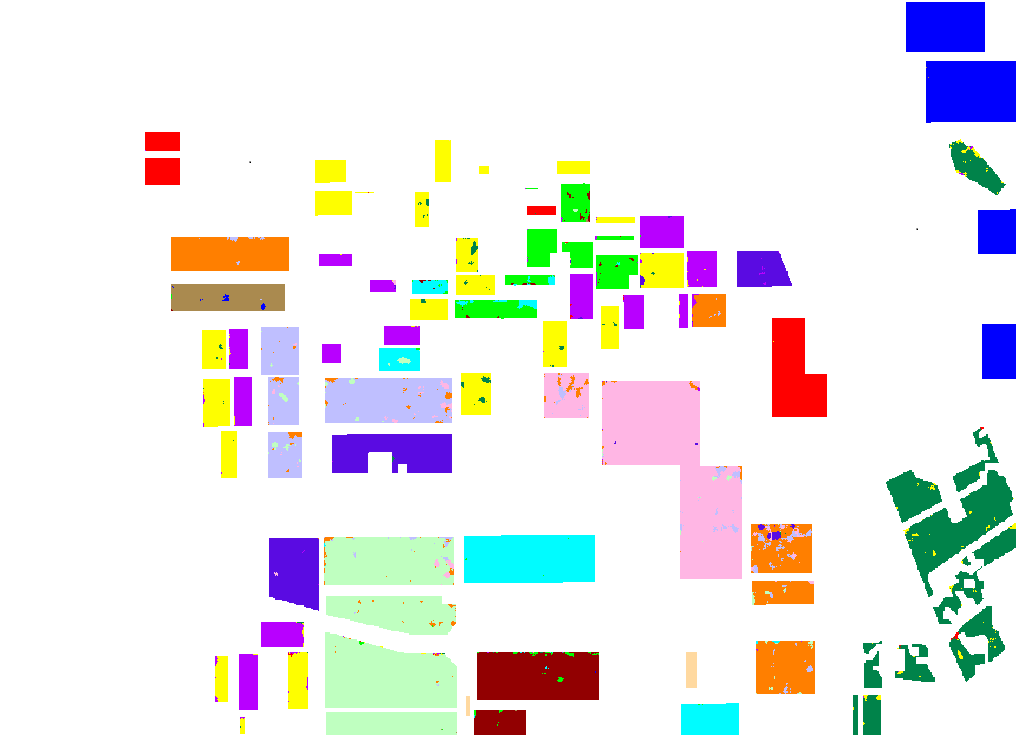
\includegraphics[width=4.74cm]{pic/chapter3/fle/CNN-T.png}
  }
  \subfloat[]{
    \label{fig:fle_P}
    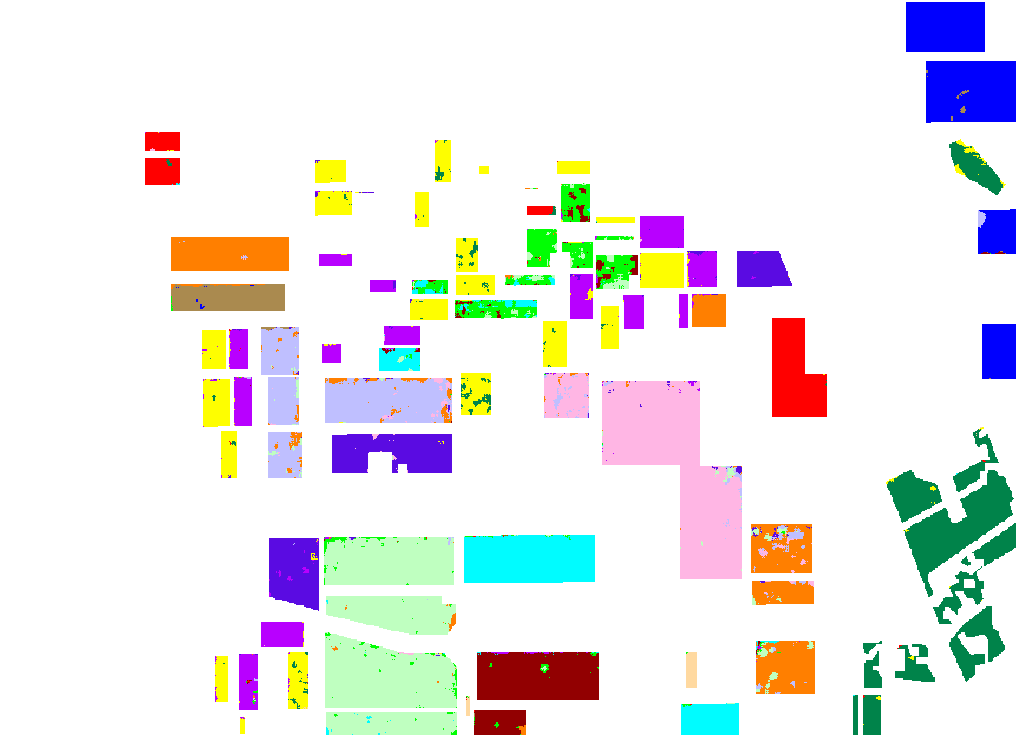
\includegraphics[width=4.74cm]{pic/chapter3/fle/CNN-P.png}
  }
  \subfloat[]{
    \label{fig:fle_F}
    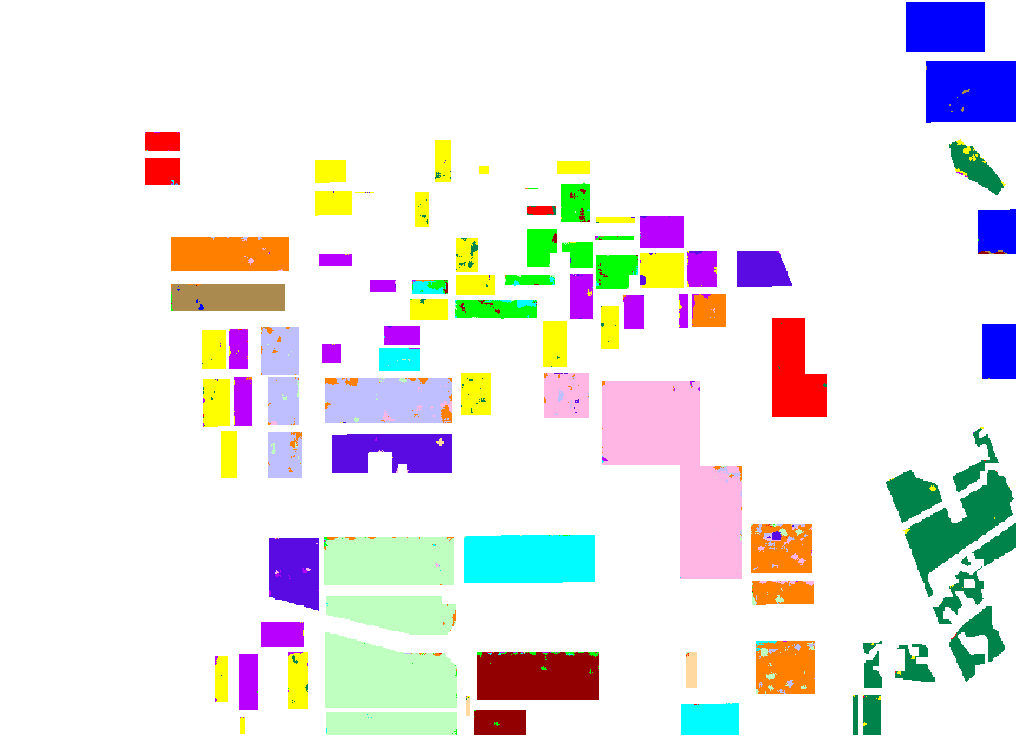
\includegraphics[width=4.74cm]{pic/chapter3/fle/CNN-F.png}
  }

  \subfloat[]{
    \label{fig:fle_SE}
    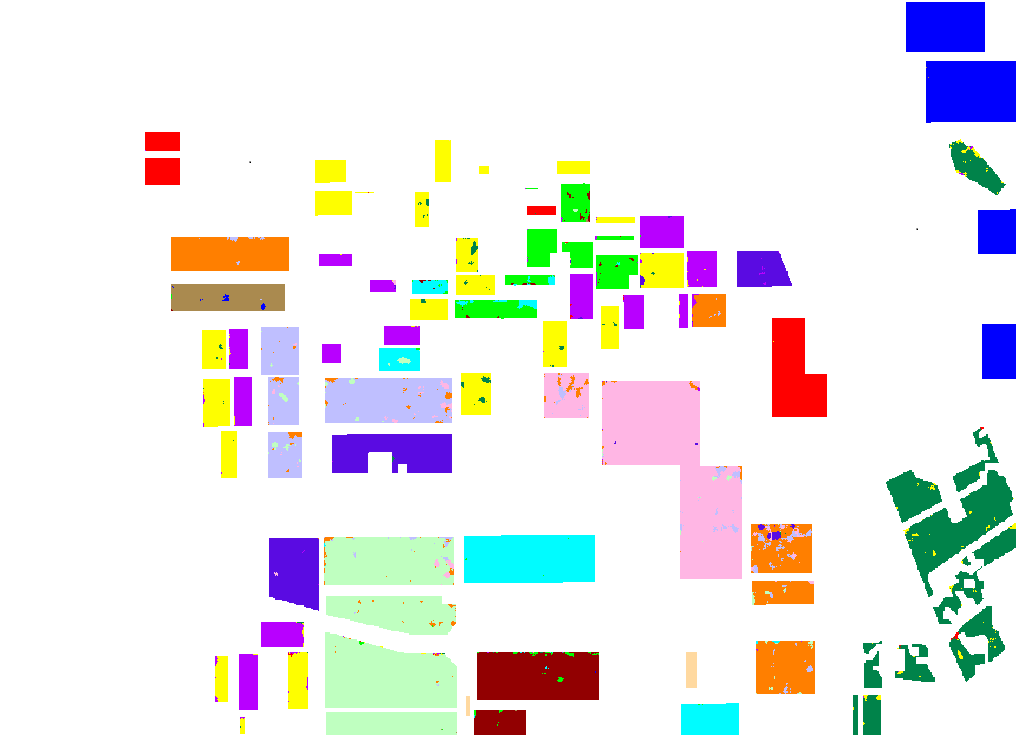
\includegraphics[width=4.74cm]{pic/chapter3/fle/CNN-T.png}
  }
  \subfloat[]{
    \label{fig:fle_CBAM}
    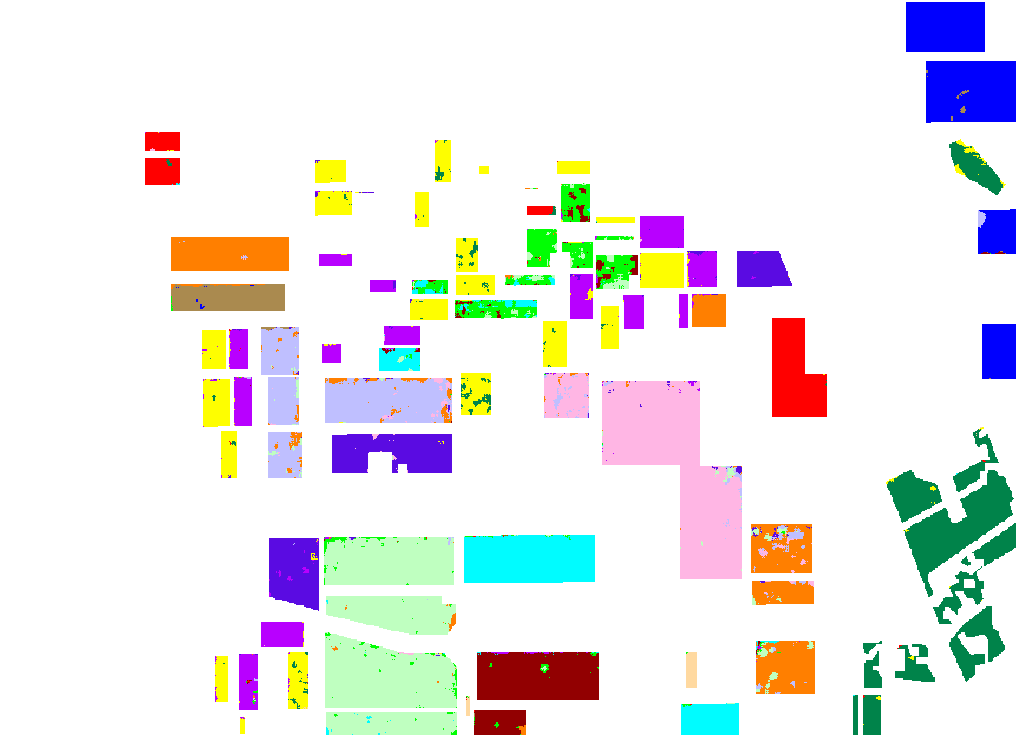
\includegraphics[width=4.74cm]{pic/chapter3/fle/CNN-P.png}
  }
  \subfloat[]{
    \label{fig:fle_DP}
    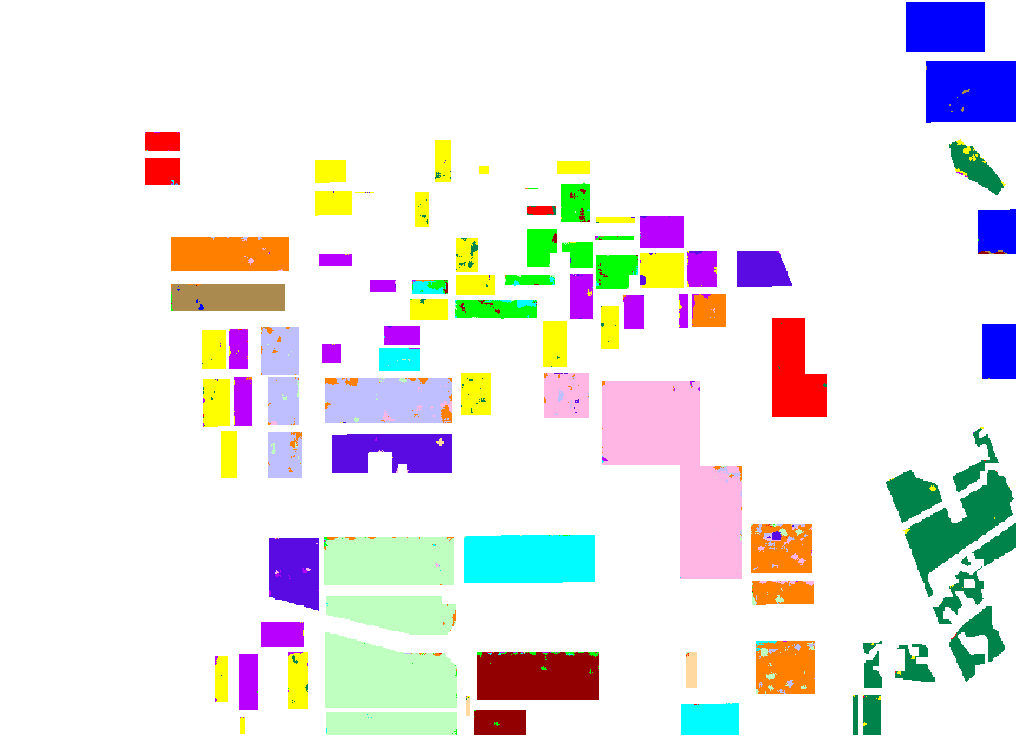
\includegraphics[width=4.74cm]{pic/chapter3/fle/CNN-F.png}
  }
  \caption{AIRSAR Flevoland地区数据分类可视化结果图。(a) CNN-T; (b) CNN-P; (c) CNN-F; (d) CNN-SE; (e) CNN-CBAM; (f) 本章方法}
  \label{fig:fle_res}
\end{figure}

为了进一步探索极化信息提取模块的性能,引入t-SNE(t-distributed Stochastic Neighbor Embedding)\citing{}特征分布图作为衡量极化信息提取模块的可视化评估指标。t-SNE是一种非线性降维技术,能够有效地将高维数据映射到二维或三维空间,以便更直观地观察样本在特征空间的分布。

图\ref{fig:fle-tSNE}展示了不同方法特征特征使用t-SNE可视化的分布情况。根据图\ref{fig:fle_t_t}、图\ref{fig:fle_t_p}和图\ref{fig:fle_t_f}所展示的仅散射特征、仅分解特征和直接堆叠特征三种不同的特征分布情况,可以看出大多数类别相互之间有交叠的情况,并且类内的样本分布较为散乱,因而容易造成类间错分的情况,导致分类性能优先。而图\ref{fig:fle_t_se}和图\ref{fig:fle_t_cbam}展示的使用经典的注意力信息提取方法的特征分布图,可以看出经典的注意力方法由于没有考虑极化SAR的数据特性,不同类别之间的重叠情况依然存在,并且类内样本特征分布散乱,证明了在信息提取时不考虑极化SAR数据特征对分类模型的性能提升是有限的。根据图\ref{fig:fle_t_dp}所展示的基于双通道注意力的极化信息提取方法的特征分布图,可以看到相比于其他的特征分布情况,类间的交叠现象有了明显的改善,同时类内样本特征分布更加紧凑,提升类间可分性,进而带来分类性能上的提升。


\begin{figure}[ht]
  \subfloat[]{
    \label{fig:fle_t_t}
    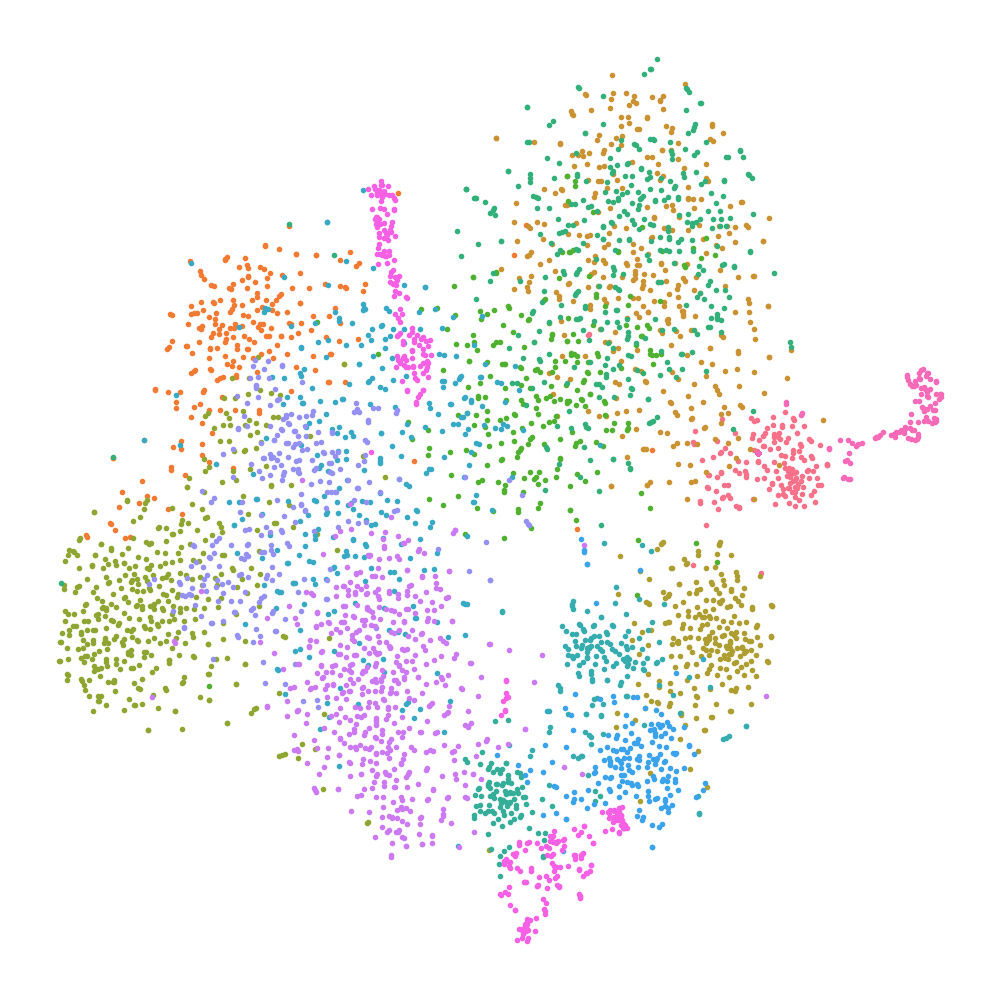
\includegraphics[width=4.74cm]{pic/chapter3/fle/tSNE-T.png}
  }
  \subfloat[]{
    \label{fig:fle_t_p}
    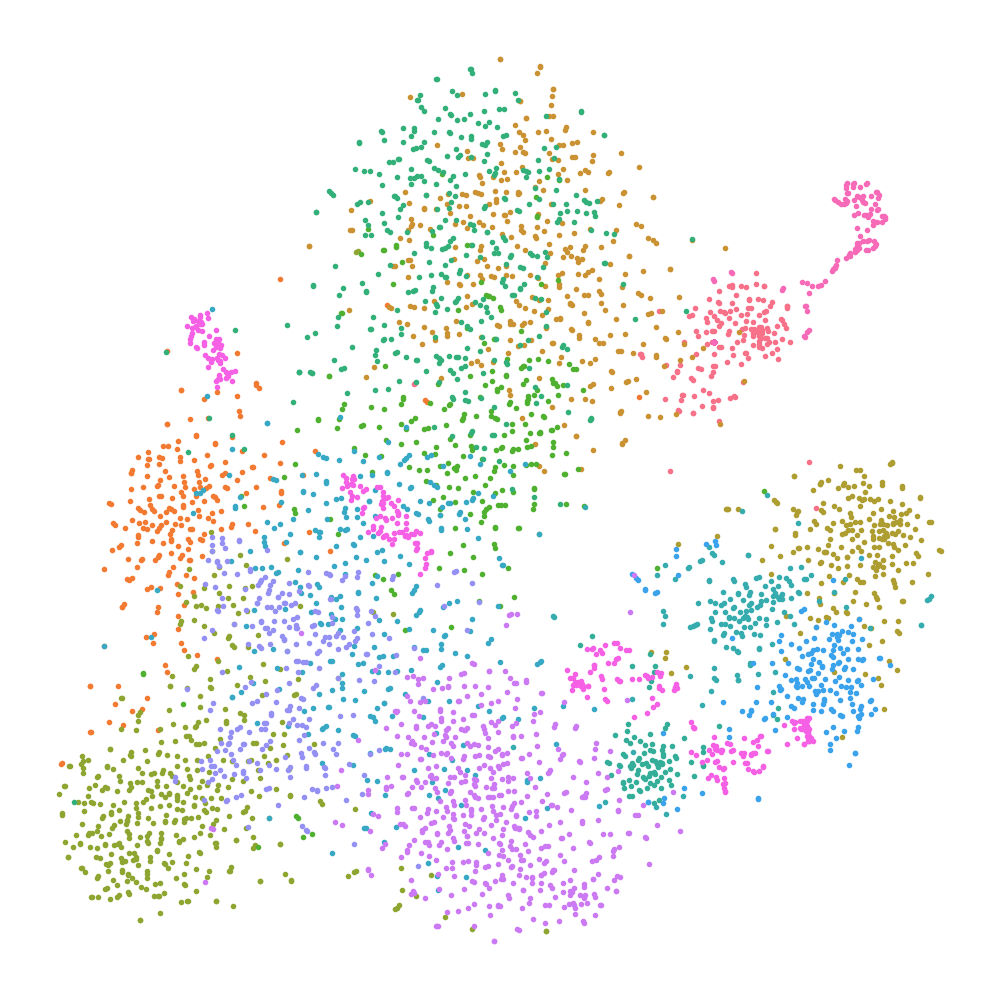
\includegraphics[width=4.74cm]{pic/chapter3/fle/tSNE-P.png}
  }
  \subfloat[]{
    \label{fig:fle_t_f}
    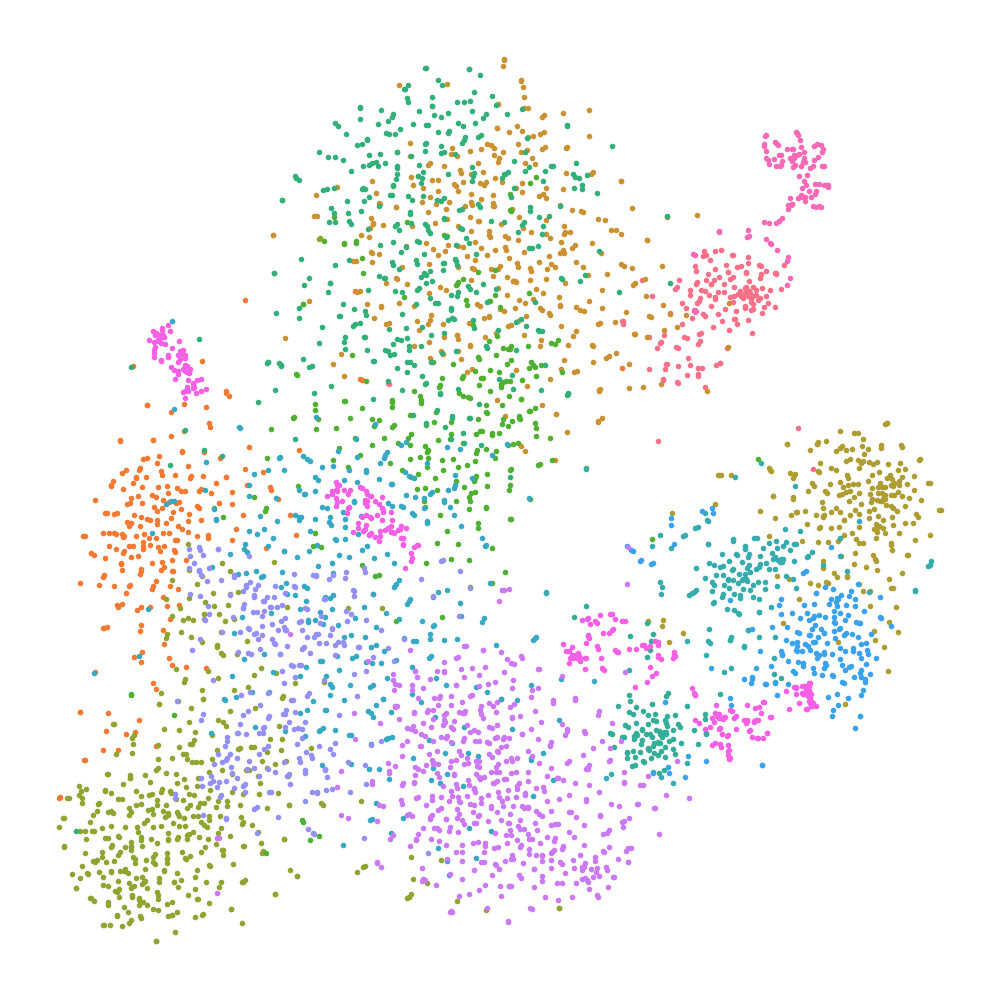
\includegraphics[width=4.74cm]{pic/chapter3/fle/tSNE-F.png}
  }

  \subfloat[]{
    \label{fig:fle_t_se}
    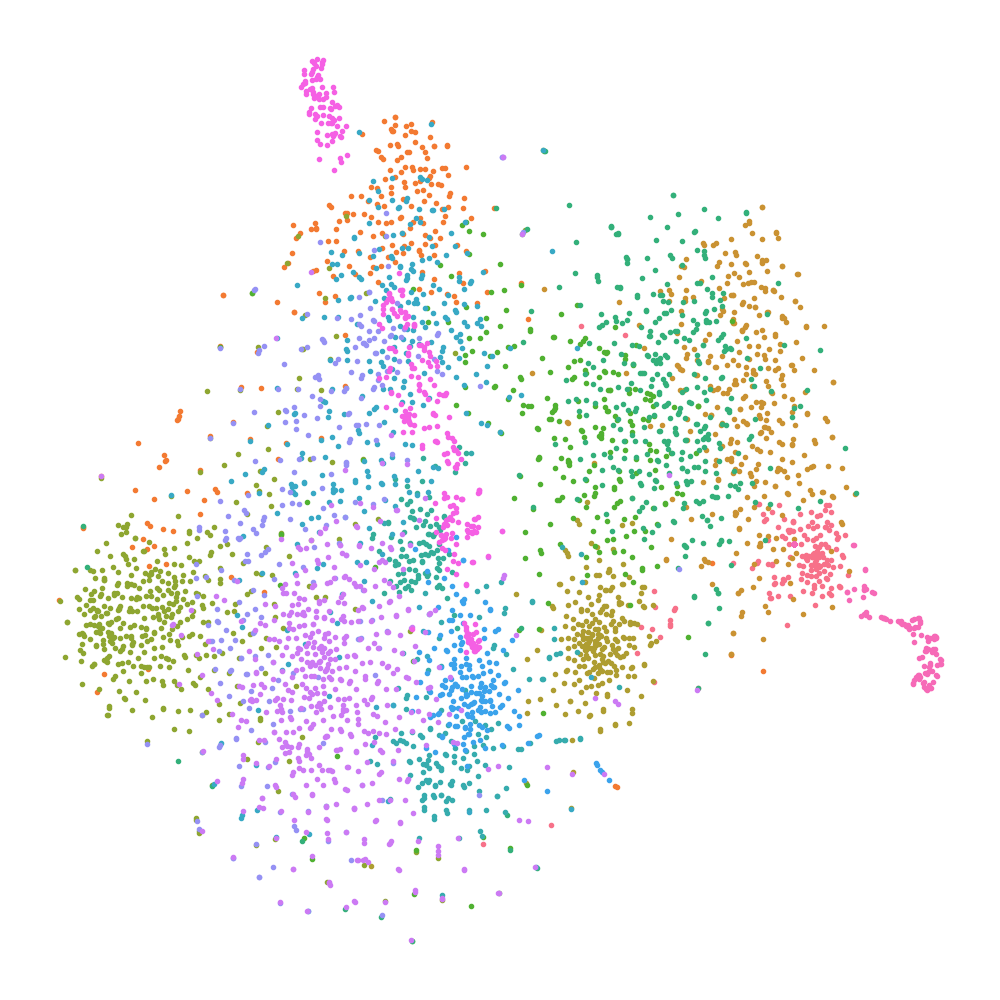
\includegraphics[width=4.74cm]{pic/chapter3/fle/tSNE-SE.png}
  }
  \subfloat[]{
    \label{fig:fle_t_cbam}
    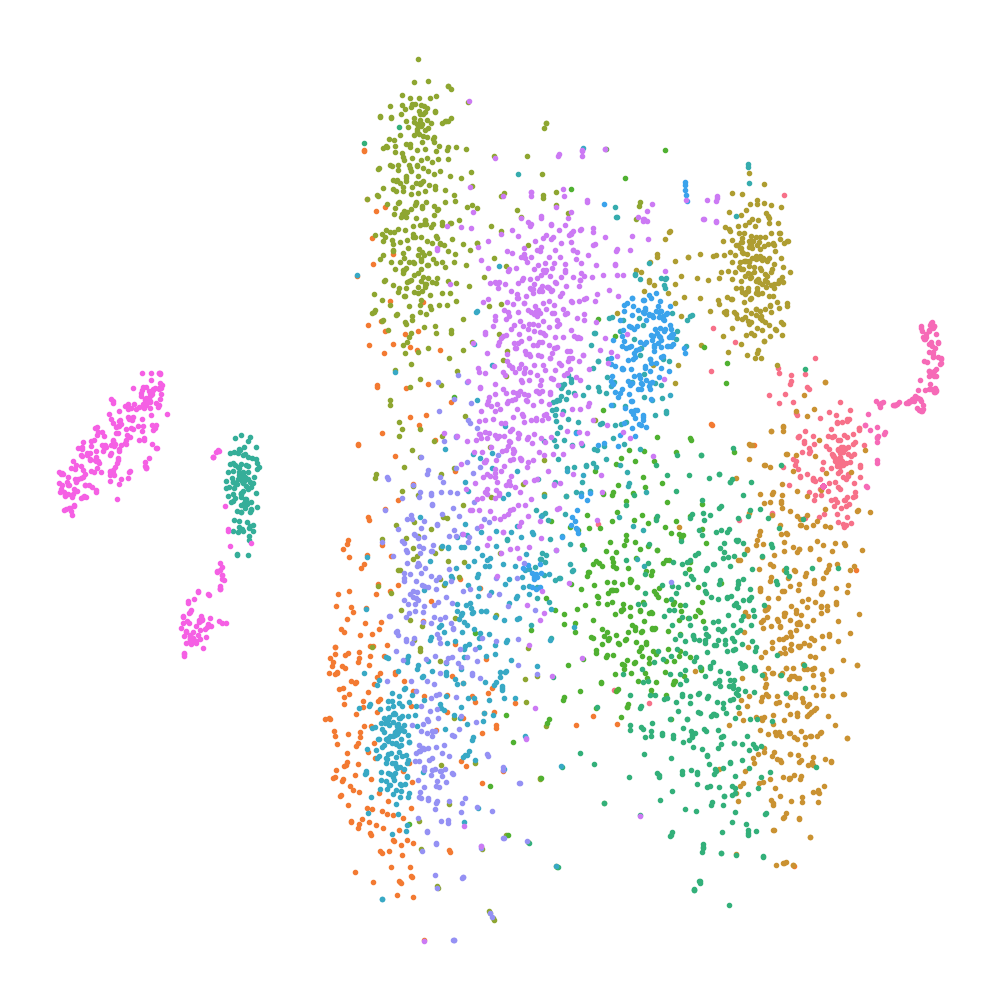
\includegraphics[width=4.74cm]{pic/chapter3/fle/tSNE-CBAM.png}
  }
  \subfloat[]{
    \label{fig:fle_t_dp}
    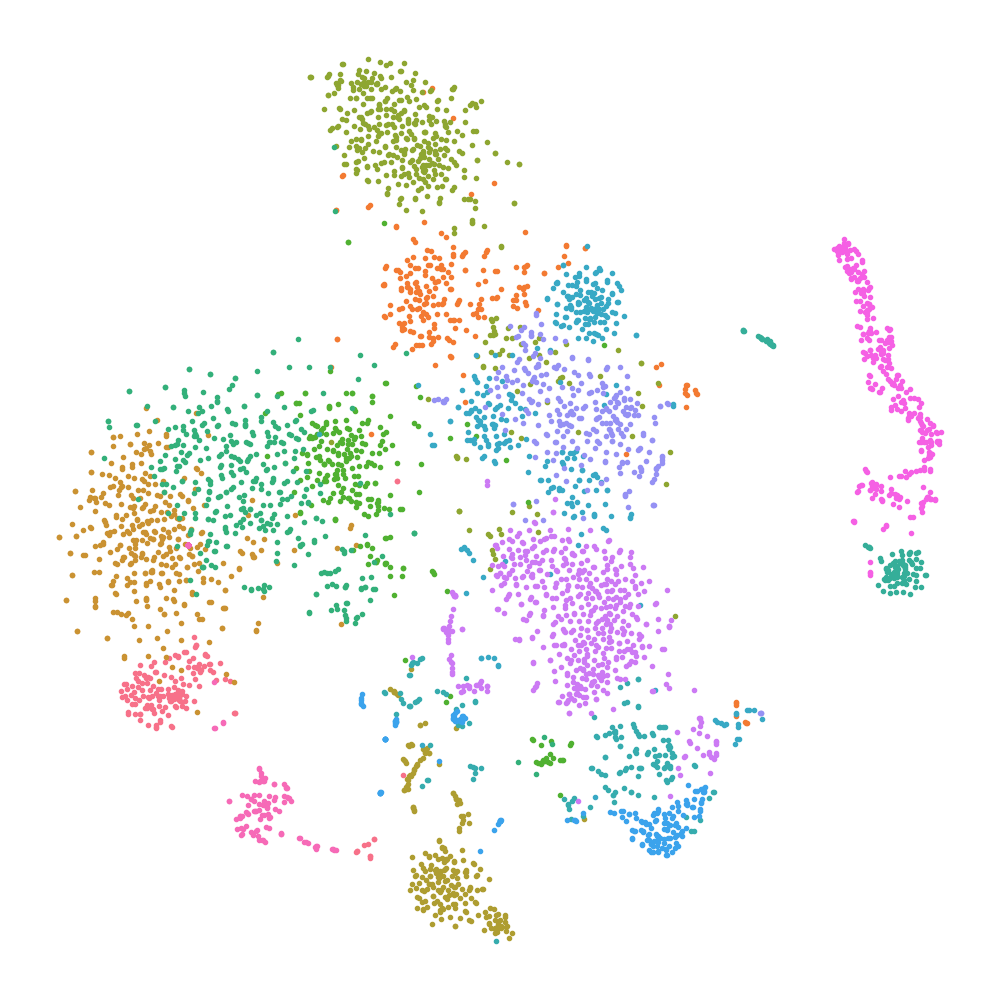
\includegraphics[width=4.74cm]{pic/chapter3/fle/tSNE-DP.png}
  }

  \subfloat[]{
    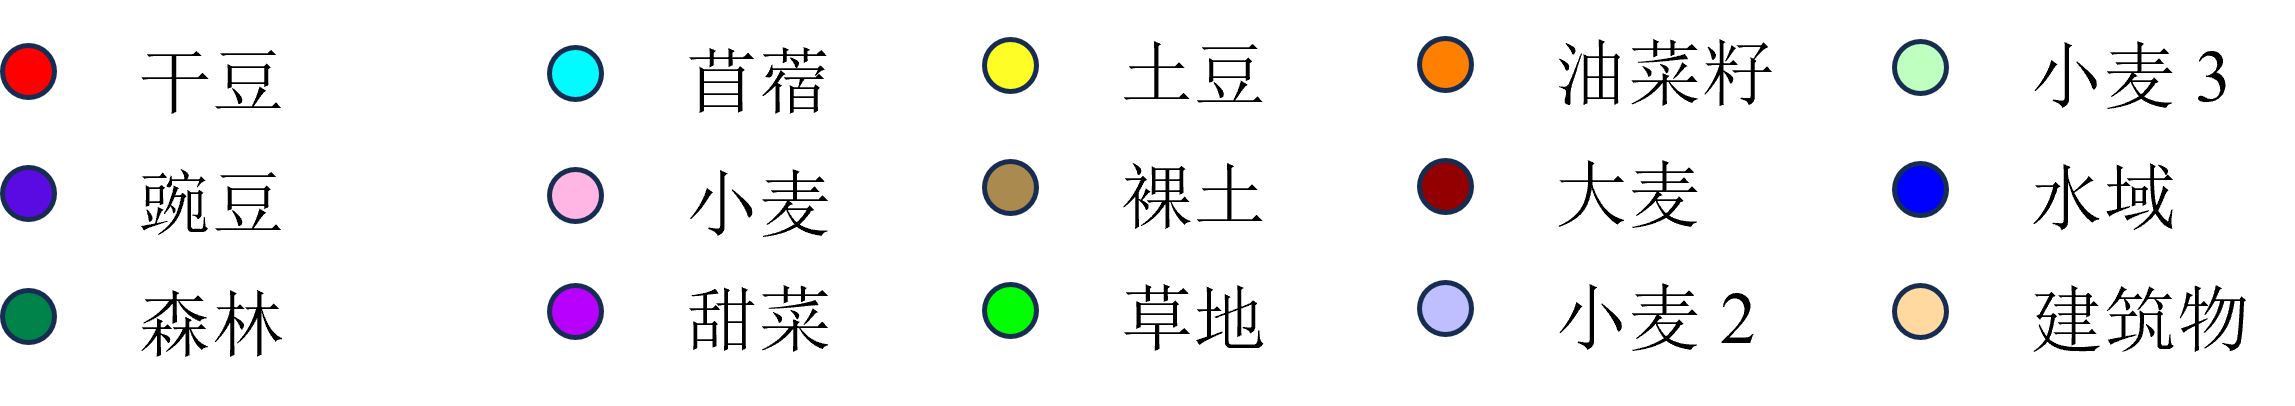
\includegraphics[width=10.04cm]{pic/chapter3/fle/tSNE-label.png}
  }
  \caption{AIRSAR Flevoland地区数据不同方法特征分布。((a) CNN-T; (b) CNN-P; (c) CNN-F; (d) CNN-SE; (e) CNN-CBAM; (f) 本章方法; (g) 颜色与类别对应关系}
  \label{fig:fle-tSNE}
\end{figure}

表\ref{tab:fle_result}展示了不同方法的分类数值结果。仅使用散射特征的分类方法,在草地和建筑物区域的分类准确率较低,分别为89.41\%和91.17\%,这可能是因为仅使用相干矩阵作为极化特征的分类方法,并不能完全反应这两类地物目标的散射特性,导致分类准确率较低。仅使用目标分解特征作为特征的分类方法,在小麦区域取得了较好的分类情况,这是因为目标分解特征中包含有具体物理意义的极化表征,但是在建筑物油菜籽区域的分类准确率较低,反映了目标分解特征与散射特征相互补充,都是必不可少的极化特征表示方法。直接堆叠极化特征的分类方法在分类总体准确率、平均准确率以及大麦等区域准确率反而下降,这表明了直接堆叠极化特征导致特征维数增加,分类器无法有效分清两种类型的主次关系,导致分类准确率有所下降。根据基于经典注意力方法的分类结果,尽管分类结果准确率指标有小幅度提升,但是实质上没有明显的数值提升,也是因为经典的注意力方法并没有考虑极化特征的特点,并不适用于极化信息提取领域。根据本章方法的分类数值结果,在大多数的类别都具有最高的分类准确率,并且在总体准确率、平均准确率、Kappa系数分别提升1.02\%、0.8\%和1.14\%,表明了基于双通道注意力的极化信息提取方法对于极化SAR目标分类具有优势,验证了本章方法的有效性和优越性。

\begin{table}[ht!]
  \label{tab:fle_res}
  \caption{AIRSAR Flevoland地区数据分类数值结果(\%)}
  \renewcommand\arraystretch{1.0}
  \begin{tabular}{cccccccc}
    \toprule[1.5bp]
    序号                        & 类别    & CNN-T          & CNN-P          & CNN-F          & CNN-SE         & CNN-CBAM       & 本章方法           \\
    \midrule[0.75bp]
    1                         & 建筑物   & 91.17          & 90.2           & 94.01          & \textbf{99.79} & 94.14          & 97.67          \\
    2                         & 油菜籽   & 94.33          & 91.78          & 89.78          & 94.54          & 92.32          & \textbf{95.98} \\
    3                         & 甜菜    & 96.57          & 96.62          & 96.99          & 97.92          & 95.74          & \textbf{98.18} \\
    4                         & 干豆    & \textbf{99.66} & 99.26          & 98.86          & 97.08          & 98.83          & 99.15          \\
    5                         & 豌豆    & 96.72          & 97.03          & 96.54          & 99.8           & 95.72          & \textbf{98.96} \\
    6                         & 森林    & 98.13          & 97.37          & 96.42          & 98.85          & 98.61          & \textbf{98.71} \\
    7                         & 苜蓿    & 96.03          & 95.96          & 95.07          & 96.11          & 95.48          & \textbf{96.12} \\
    8                         & 土豆    & 96.61          & 97.03          & \textbf{97.54} & 97.33          & 95.59          & 97.22          \\
    9                         & 裸土    & 95.02          & 97.19          & 98.44          & 98.51          & 96.8           & \textbf{98.65} \\
    10                        & 草地    & 89.41          & 93.11          & 92.32          & 96.19          & 94.25          & \textbf{96.7}  \\
    11                        & 大麦    & 93.63          & 95.45          & 87.34          & 95.64          & 89.34          & \textbf{98.11} \\
    12                        & 水域    & 99.94          & 99.7           & 99.66          & 93.3           & 99.83          & \textbf{99.96} \\
    13                        & 小麦 1  & 97.53          & 96.74          & 97.36          & 97.27          & 97.6           & \textbf{97.65} \\
    14                        & 小麦 2  & 93.62          & \textbf{94.48} & 94.21          & 97.53          & 92.25          & 94.46          \\
    15                        & 小麦 3  & 96.88          & 97.05          & 98.06          & 94.85          & 98.51          & \textbf{99.14} \\
    \midrule[0.75bp]
    \multicolumn{2}{c}{OA}    & 96.4  & 96.41          & 95.9           & 96.76          & 96.13          & \textbf{97.82}                  \\
    \multicolumn{2}{c}{AA}    & 95.68 & 95.93          & 95.51          & 96.98          & 95.67          & \textbf{97.78}                  \\
    \multicolumn{2}{c}{Kappa} & 96.07 & 96.08          & 95.53          & 96.48          & 95.77          & \textbf{97.62}                  \\
    \bottomrule[1.5bp]
  \end{tabular}
\end{table}

图\ref{fig:fle_conf_matrix}展示了本章方法分类结果的混淆矩阵可视化图。从图中可以看到,混淆矩阵的可视化结果显示本章方法在对角线上具有较高的主对角元素,说明在大多数类别上取得了良好的分类性能。

\begin{figure}[h]
  \centering
  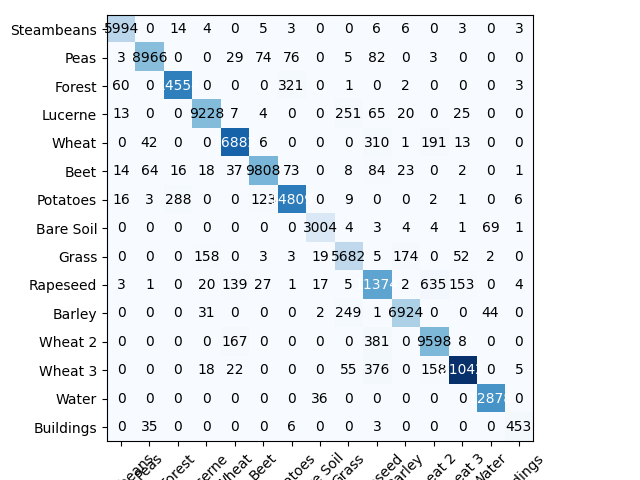
\includegraphics[width=10.4cm]{pic/chapter3/fle/conf-matrix.png}
  \caption{本章方法在Flevoland图像中分类结果混淆矩阵图}
  \label{fig:fle_conf_matrix}
\end{figure}


\subsection{E-SAR Oberpfaffenhofen数据实验}
该数据集是通过E-SAR机载平台在德国Oberpfaffenhofen地区拍摄获取到的L波段极化SAR数据。该数据集经过多视处理,具有高质量的全极化信息,是极化SAR目标分类研究的经典数据集之一。数据集在方位向和距离向具有$3m \times 3m$的分辨率,大小为$1300 \times 1200$,总计包含三种类型的地物目标,分别是:建筑、林地和开放区域。图\ref{fig:ober_pauli}展示了该数据集的Pauli伪彩色图像,图\ref{fig:ober_gt}展示了该数据集的人工标记的地面真值参考图。地面真值图中黑色的区域表示未标记的区域。表\ref{fig:ober_label}展示了各类地物目标样本数量情况。

\begin{figure}[ht]
  \subfloat[]{
    \label{fig:ober_pauli}
    \includegraphics[width=4.04cm]{pic/chapter3/ober/Pauli.png}
  }
  \subfloat[]{
    \label{fig:ober_gt}
    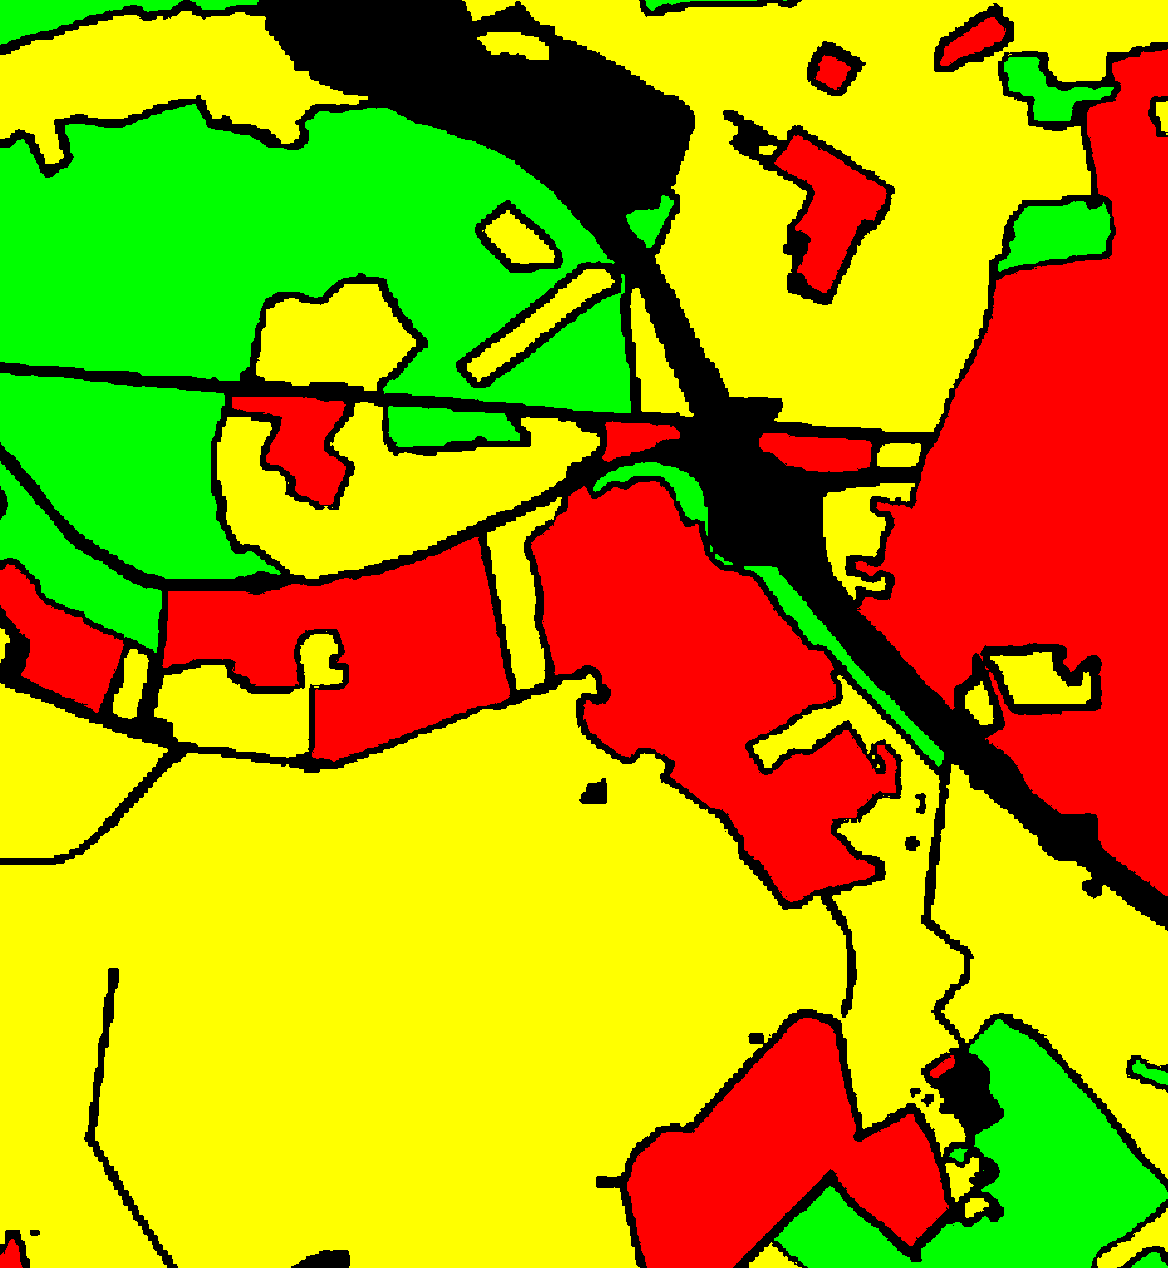
\includegraphics[width=4.04cm]{pic/chapter3/ober/gt.png}
  }

  \subfloat[]{
    \label{fig:ober_label}
    
\includegraphics[width=7.04cm]{pic/chapter3/ober/label.png}
  }
  \caption{E-SAR Oberpfaffenhofen区域数据。(a)Pauli分解伪彩色图像;(b)实验数据地面真值;(c)颜色与类别对应关系}
\end{figure}

\begin{table}[ht]
  \caption{ESAR Oberpfaffenhofen数据样本数量}
  \label{tab:ober_sample}
  \centering
  \begin{tabular}{|c|c|c|c|}
    \hline
    类别 & 建筑      & 林地      & 开放区     \\ \hline
    数目 & 269,184 & 388,503 & 779,962 \\ \hline
  \end{tabular}
\end{table}

图\ref{fig:ober_res}展示了不同方法的分类结果可视化图像。根据图\ref{fig:ober_T}展示的仅使用极化相干矩阵为特征的分类结果图,尽管在开放区域的分类效果较好,但是在建筑物区域存在大量被错分的样本,将建筑物区域样本错误分类为开放区域,并且错分的现象较为严重。这可能是因为仅使用极化相干矩阵作为特征时并没有完全利用其他的目标分解特征导致的,说明了综合考虑极化SAR图像中的其他极化特性和辅助特征的在分类任务中的重要性。相比之下,图\ref{fig:ober_P}与图\ref{fig:ober_F}在建筑物区域中的错分样本相对较少,但是在各类区域中也存在着部分错分的样本。其中将开放区域中的少数像素分类为建筑物的错分情况依然存在,这反映了极化目标分解特征提供的反映目标物理散射特性的信息为分类任务带来了一定的优势,是极化SAR图像中的重要的基本特征。图\ref{fig:ober_SE}和图\ref{fig:ober_CBAM}展示了基于经典注意力方法的特征表示分类结果,从结果图中可以看出,分类效果仅有微小的变化,错分像素相对减少但是依然存在,这可能是极化SAR图像与光学图像存在较大的差异,经典的注意力方法并没有考虑极化SAR图像的数据特征特点。图\ref{fig:ober_DP}展示了基于本章提出的双通道注意力极化信息提取方法的分类结果图,从图中直观可以看出,在建筑物区域的错分样本明显减少,并且每个类中的小块错误区域数量也相对减少,整体分类结果得到明显改善,证明了本章方法的有效性。

\begin{figure}[ht!]
  \subfloat[]{
    \label{fig:ober_T}
    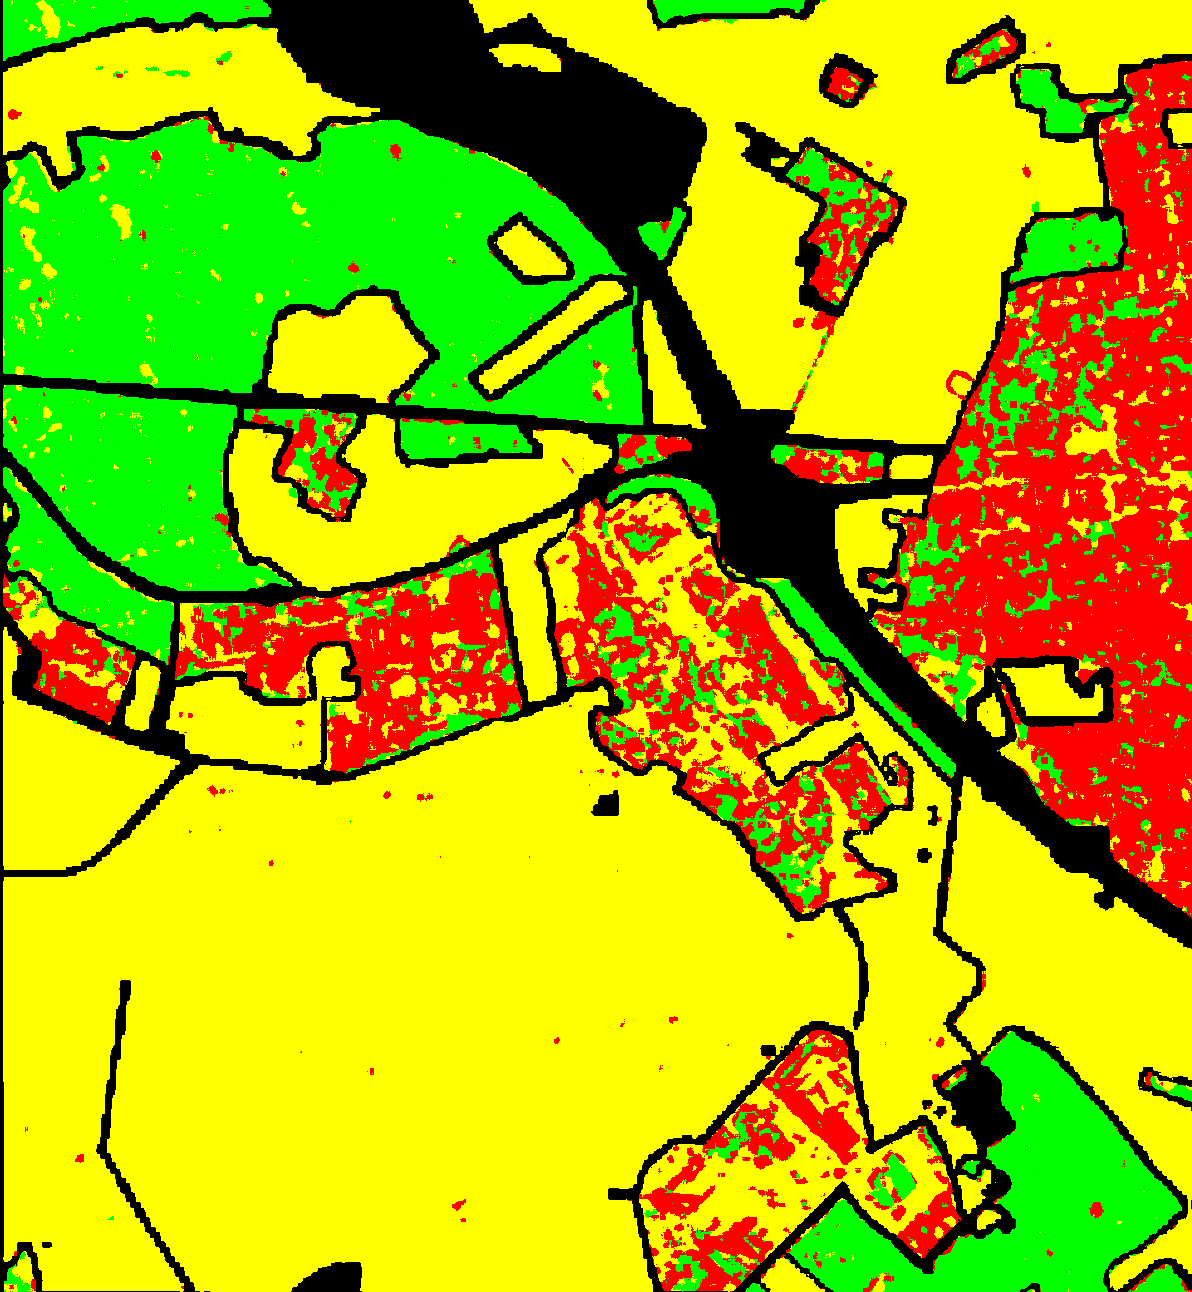
\includegraphics[width=4.04cm]{pic/chapter3/ober/CNN-T.png}
  }
  \subfloat[]{
    \label{fig:ober_P}
    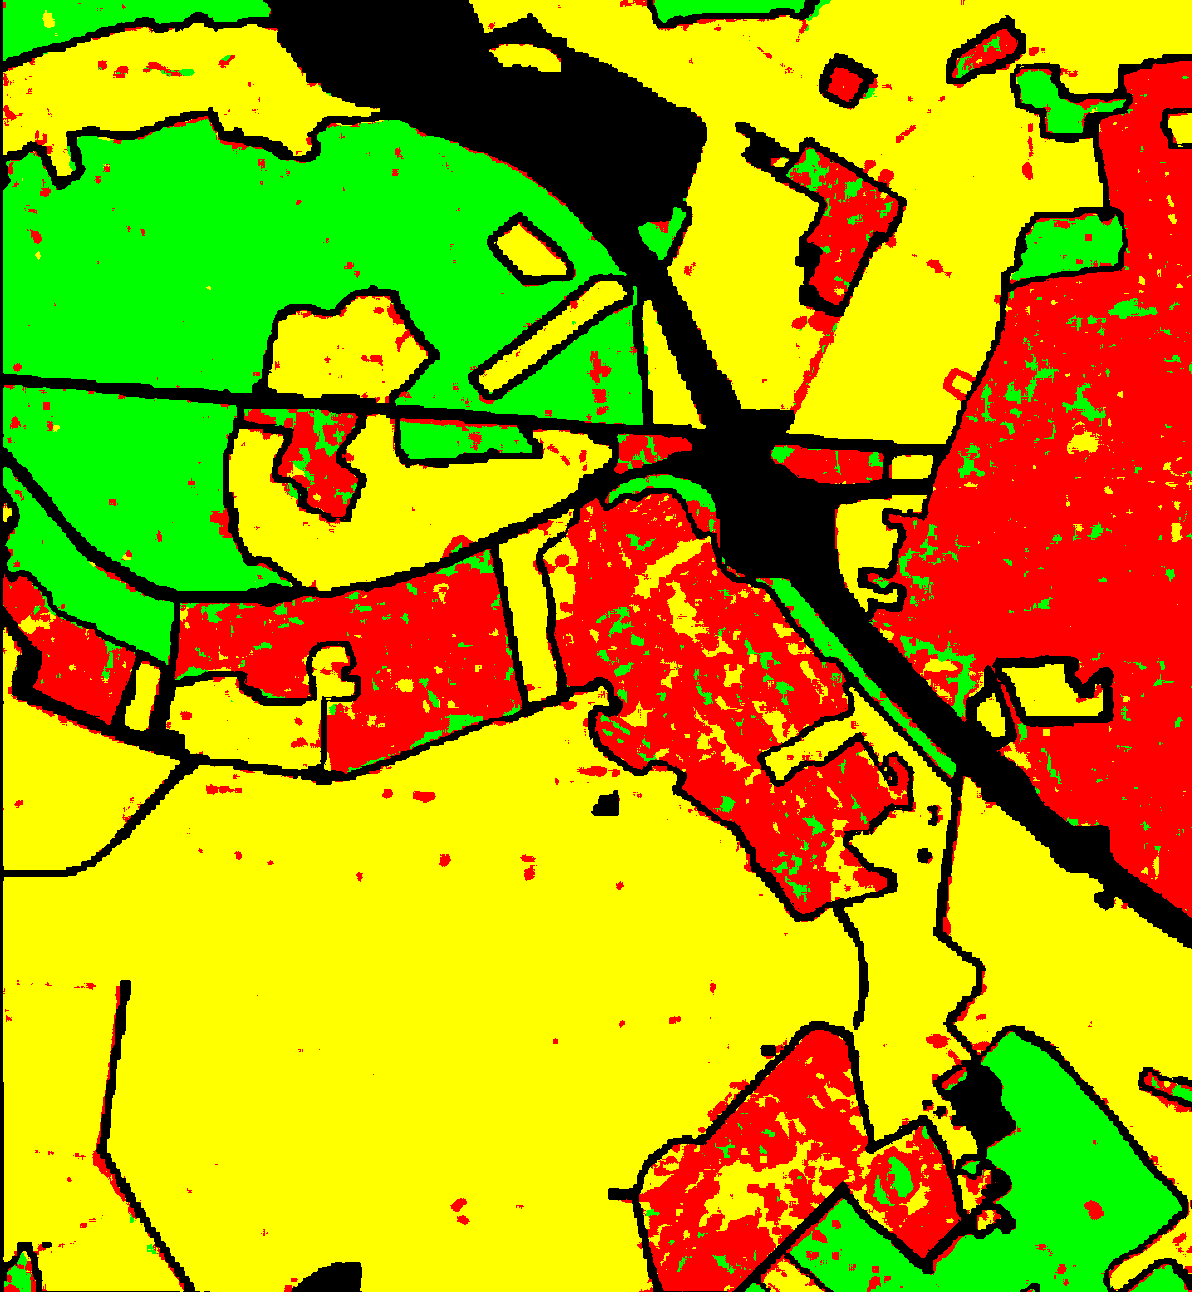
\includegraphics[width=4.04cm]{pic/chapter3/ober/CNN-P.png}
  }
  \subfloat[]{
    \label{fig:ober_F}
    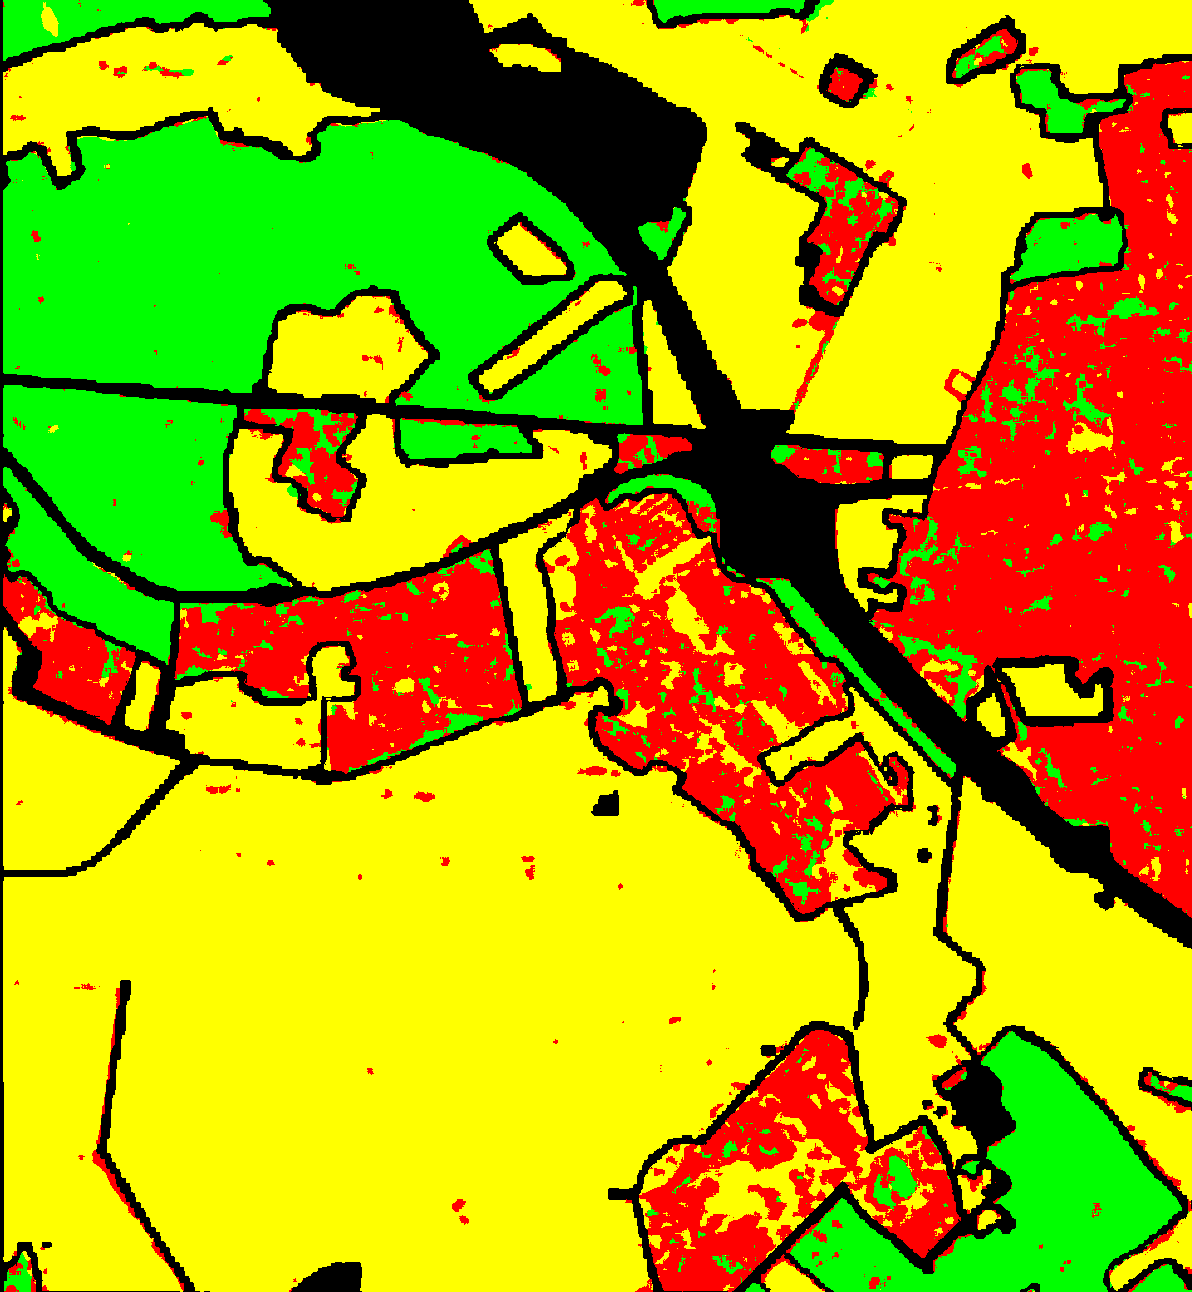
\includegraphics[width=4.04cm]{pic/chapter3/ober/CNN-F.png}
  }

  \subfloat[]{
    \label{fig:ober_SE}
    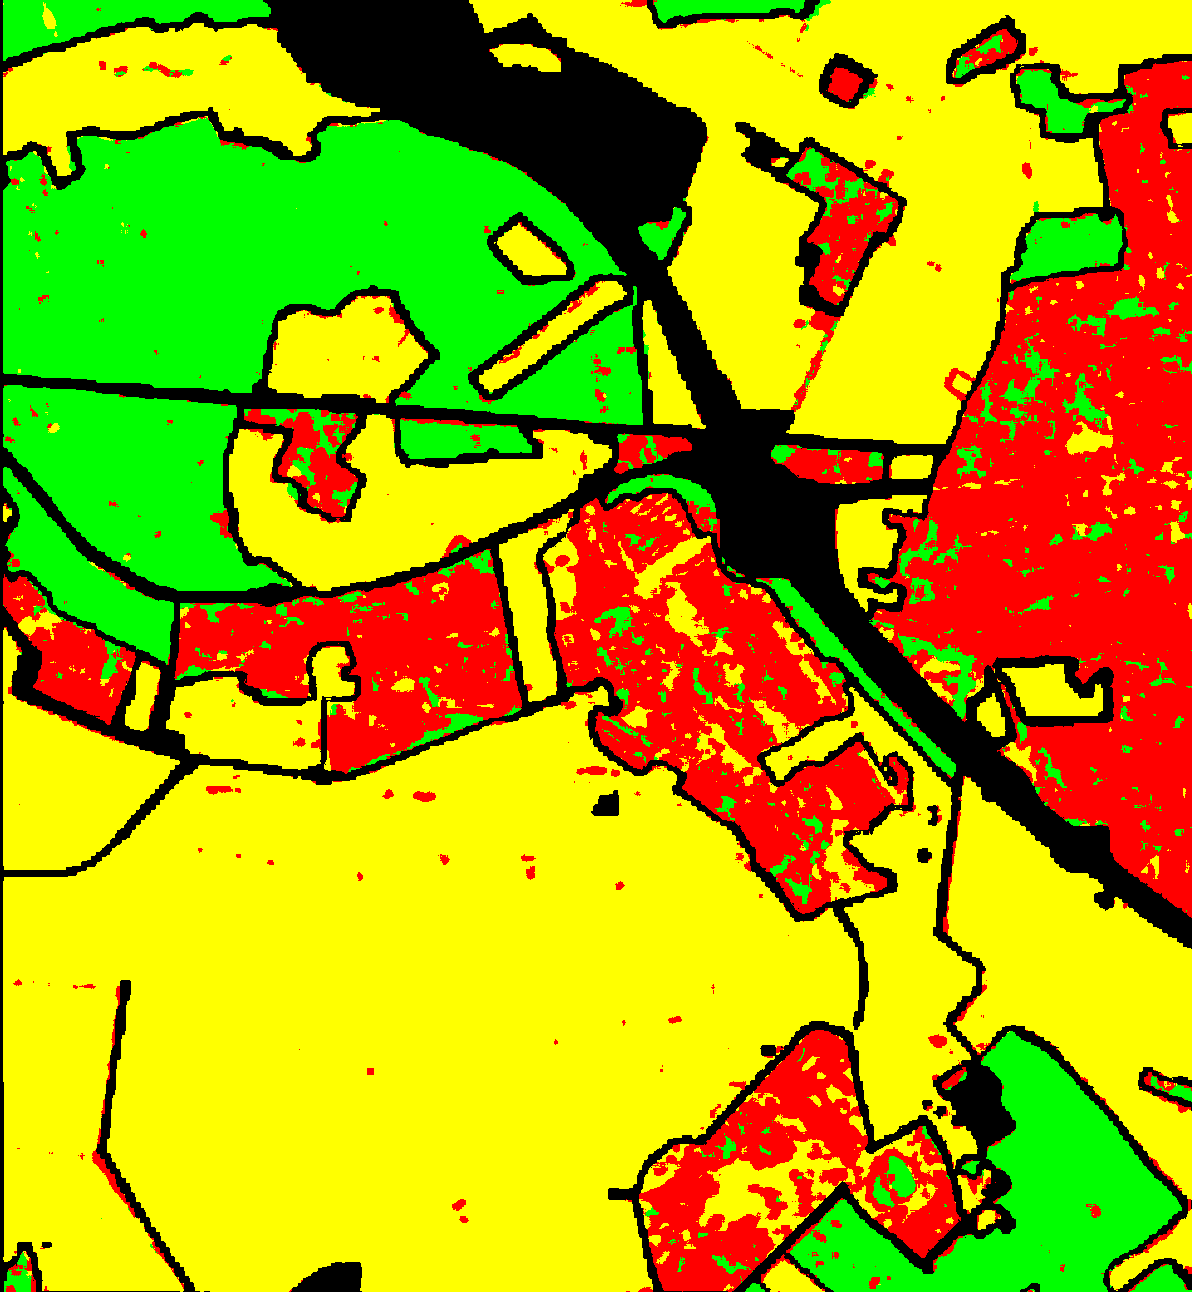
\includegraphics[width=4.04cm]{pic/chapter3/ober/CNN-SE.png}
  }
  \subfloat[]{
    \label{fig:ober_CBAM}
    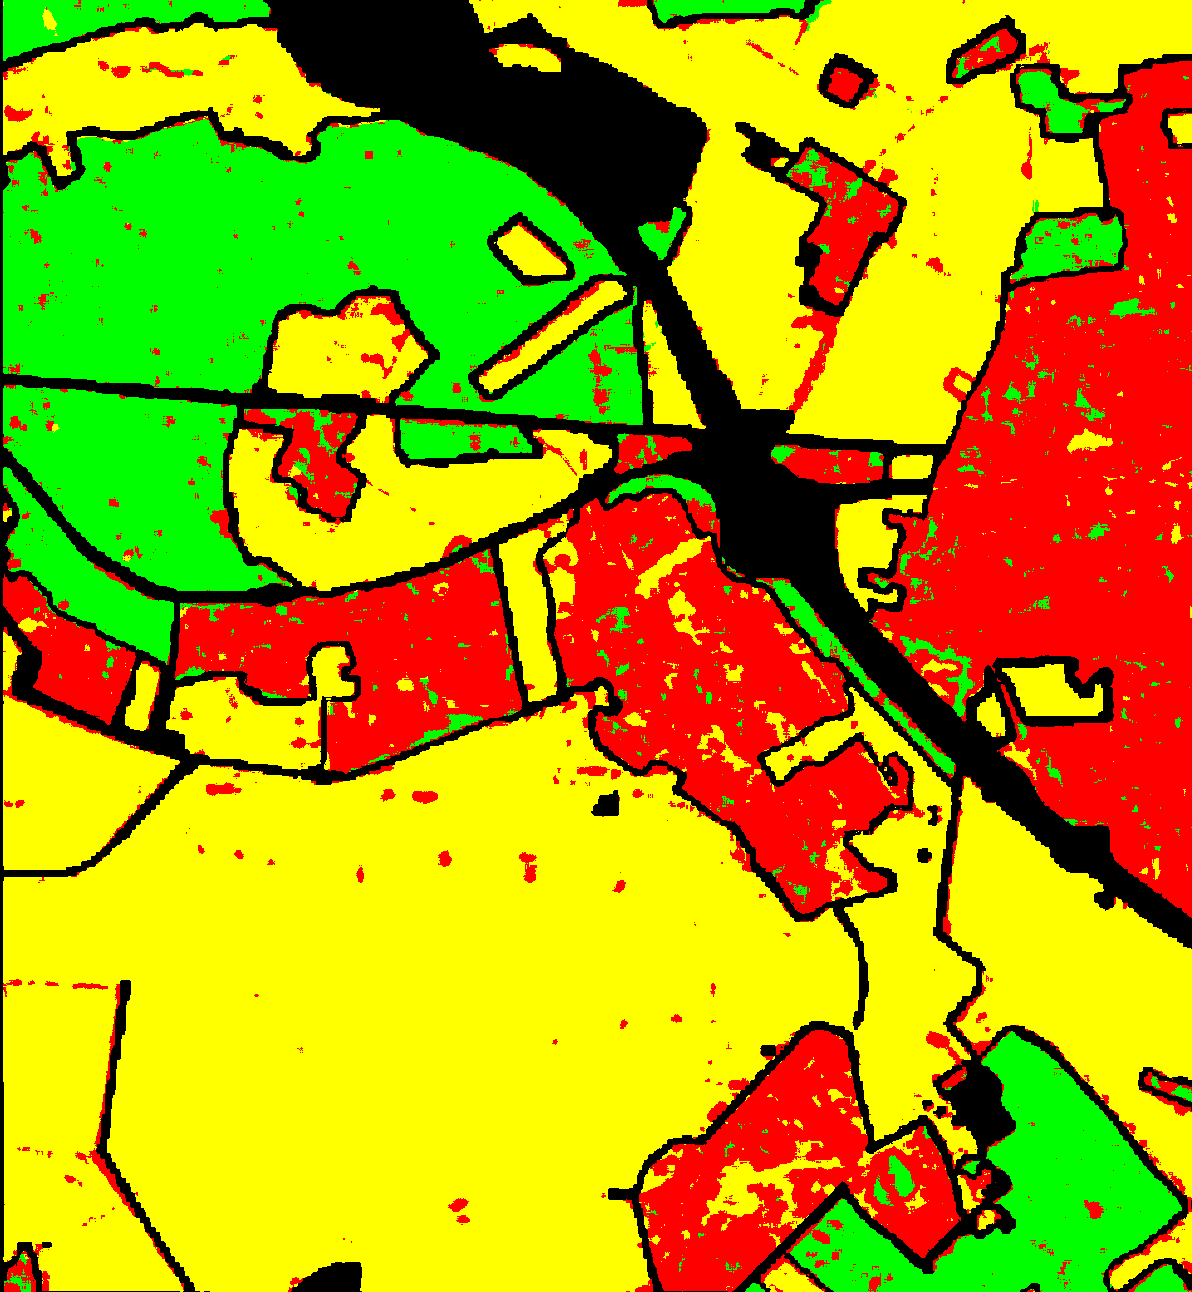
\includegraphics[width=4.04cm]{pic/chapter3/ober/CNN-CBAM.png}
  }
  \subfloat[]{
    \label{fig:ober_DP}
    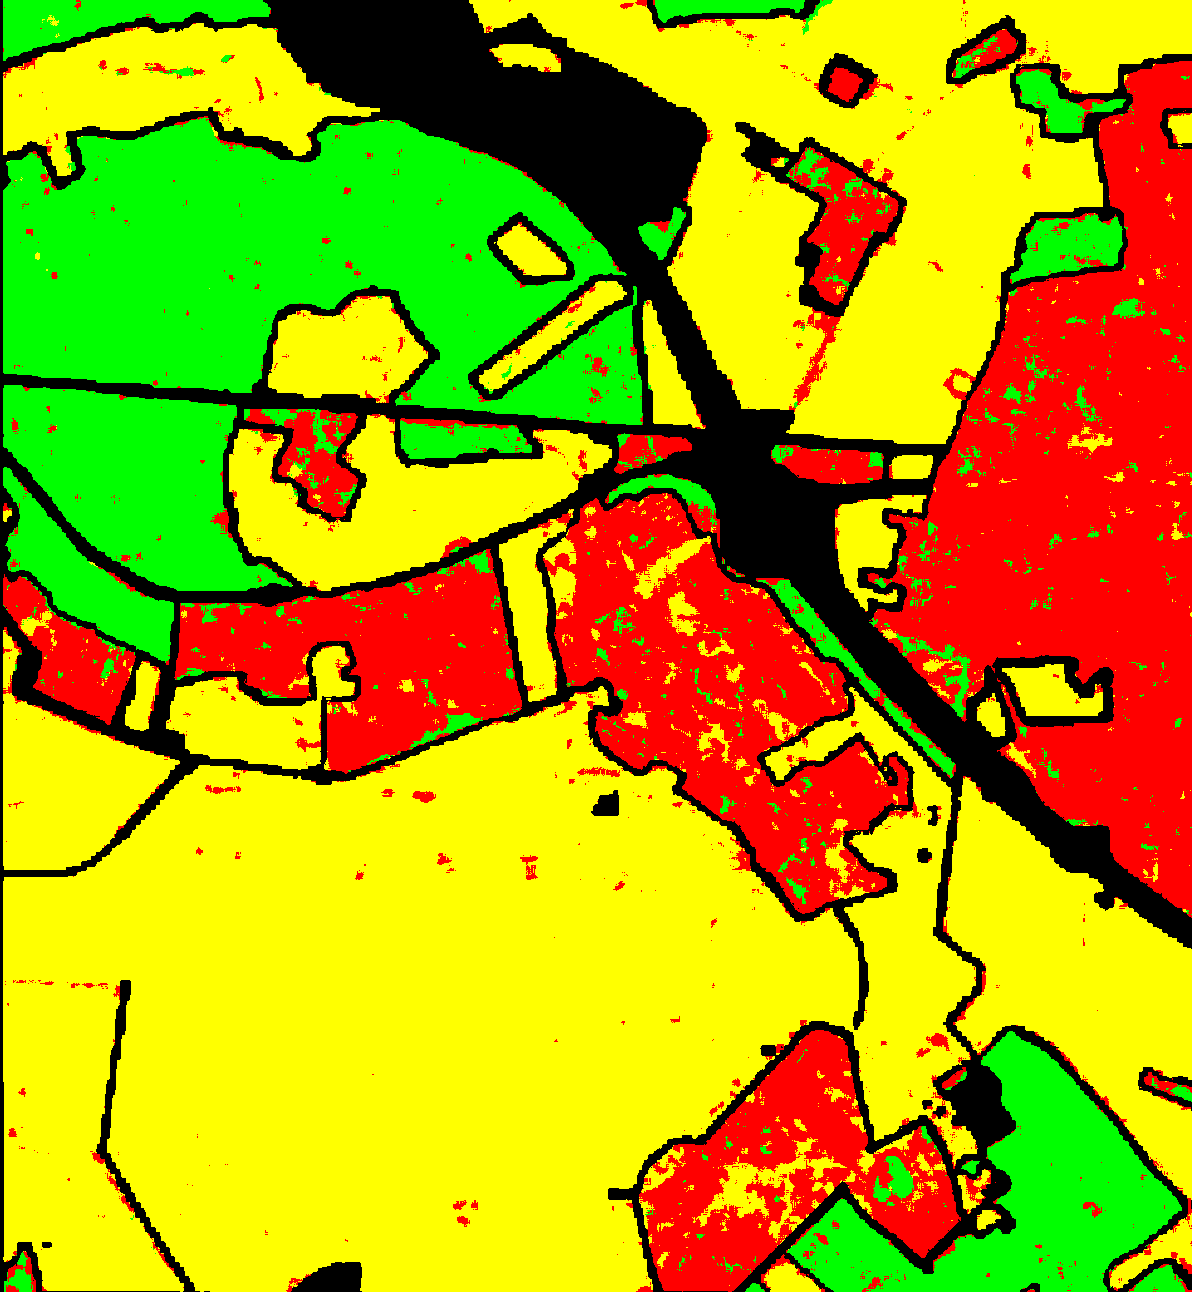
\includegraphics[width=4.04cm]{pic/chapter3/ober/CNN-DP.png}
  }

  \caption{E-SAR Oberpfaffenhofen地区数据分类可视化结果图。(a) CNN-T; (b) CNN-P; (c) CNN-F; (d) CNN-SE; (e) CNN-CBAM; (f) 本章方法}
  \label{fig:ober_res}
\end{figure}

图\ref{fig:ober-tSNE}展示了不同方法数据特征使用tSNE可视化的分布情况。根据图\ref{fig:ober_t_t}、图\ref{fig:ober_t_p}、图\ref{fig:ober_t_f}展示的仅散射特征、仅分解特征和直接堆叠的三种特征分布情况,可以看出三种特征分布情况并没有本质性的差异,尽管都可以看出各类之间存在不同的分布情况,但是也能清晰看出,类间存在分布交叠的部分,这也导致了部分样本的错分情况。根据图\ref{fig:ober_t_se}和图\ref{fig:ober_t_cbam}展示的使用经典注意力信息提取方法的特征分布图,可以看出虽然类间交叠的情况有细微改善,但是依然有大量的特征存在交叠,这也映照了分类结果改善不大的结果。图\ref{fig:ober_t_dp}展示了使用本章方法的特征分布情况,可以看出类间交叠的情况得到优化,各类之间分布间距增大,增强了类间可分性,进而带来分类性能的提升。

\begin{figure}[ht!]
  \subfloat[]{
    \label{fig:ober_t_t}
    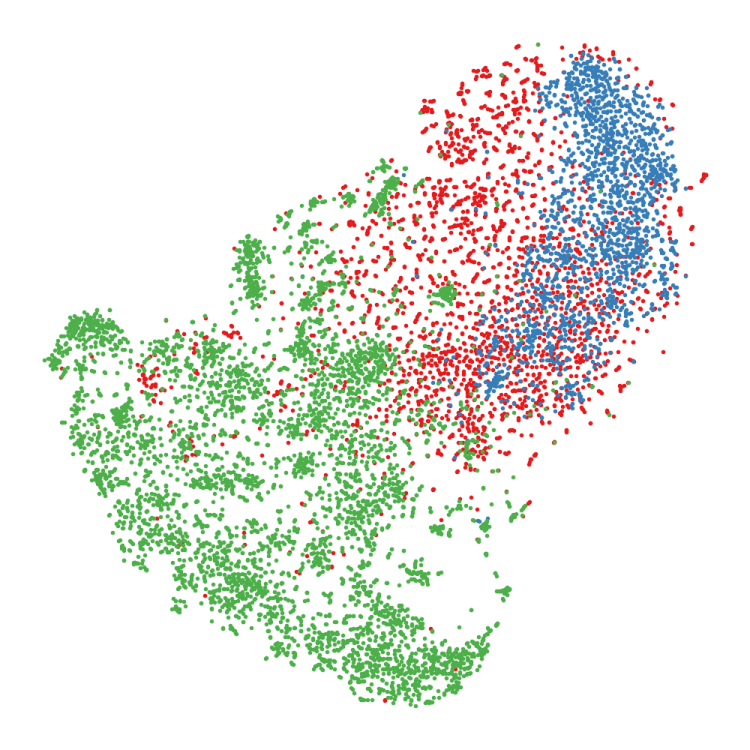
\includegraphics[width=4.04cm]{pic/chapter3/ober/tSNE-T.png}
  }
  \subfloat[]{
    \label{fig:ober_t_p}
    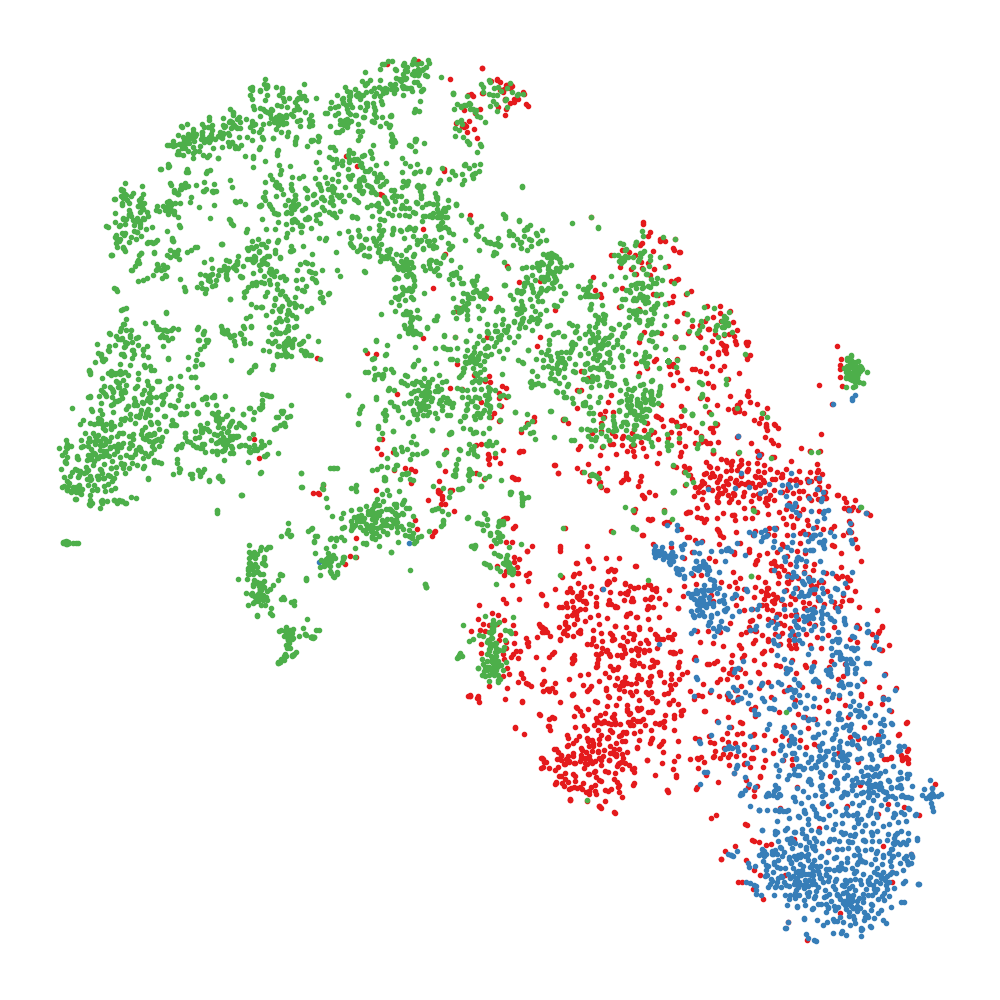
\includegraphics[width=4.04cm]{pic/chapter3/ober/tSNE-P.png}
  }
  \subfloat[]{
    \label{fig:ober_t_f}
    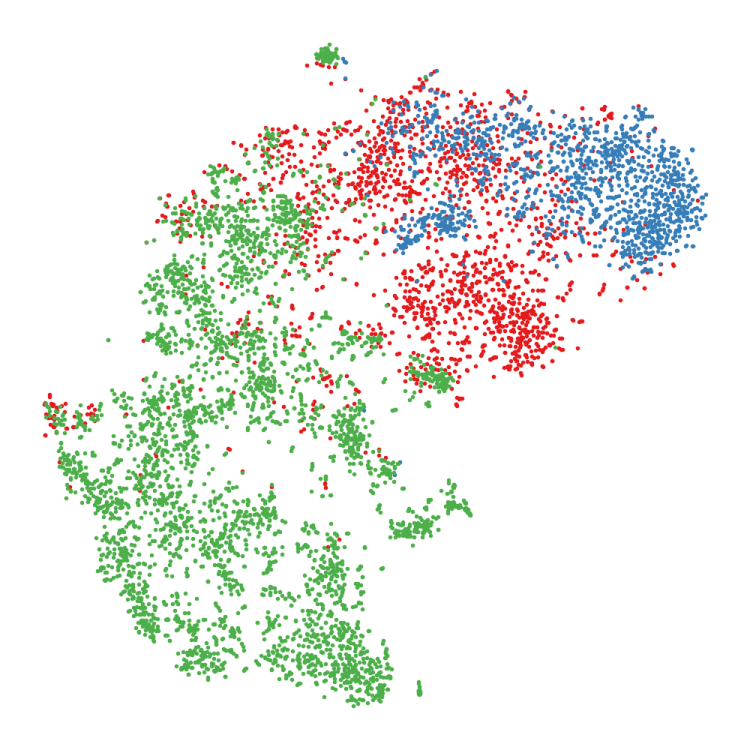
\includegraphics[width=4.04cm]{pic/chapter3/ober/tSNE-F.png}
  }

  \subfloat[]{
    \label{fig:ober_t_se}
    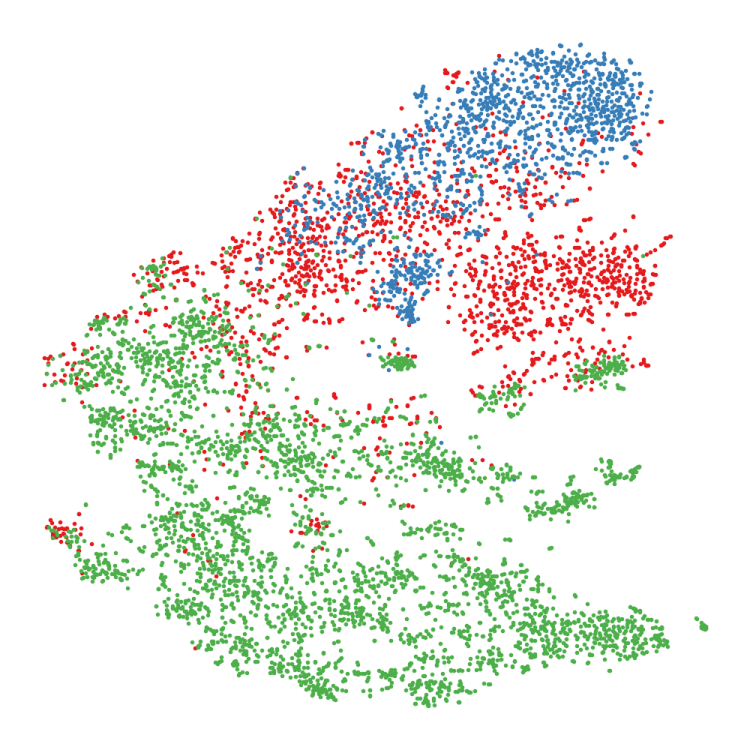
\includegraphics[width=4.04cm]{pic/chapter3/ober/tSNE-SE.png}
  }
  \subfloat[]{
    \label{fig:ober_t_cbam}
    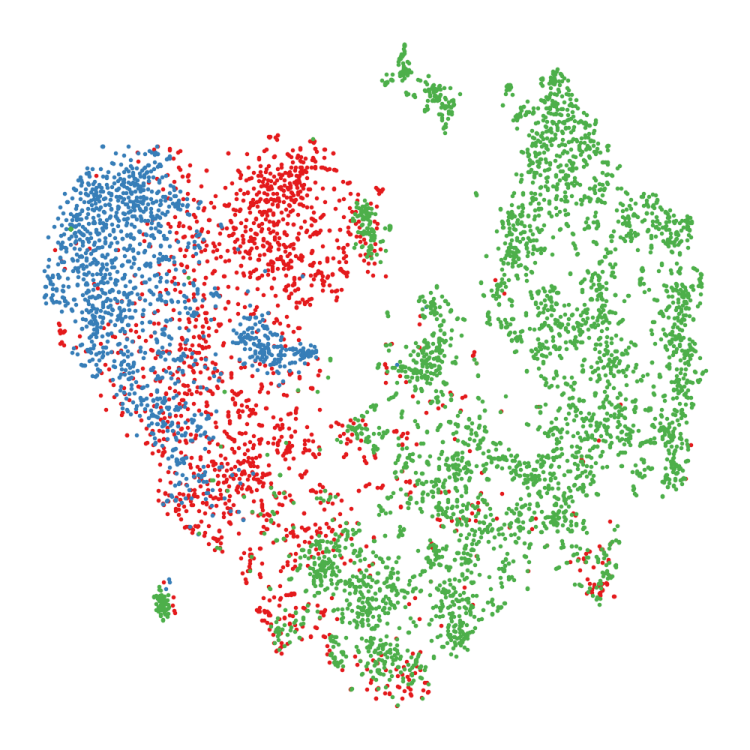
\includegraphics[width=4.04cm]{pic/chapter3/ober/tSNE-CBAM.png}
  }
  \subfloat[]{
    \label{fig:ober_t_dp}
    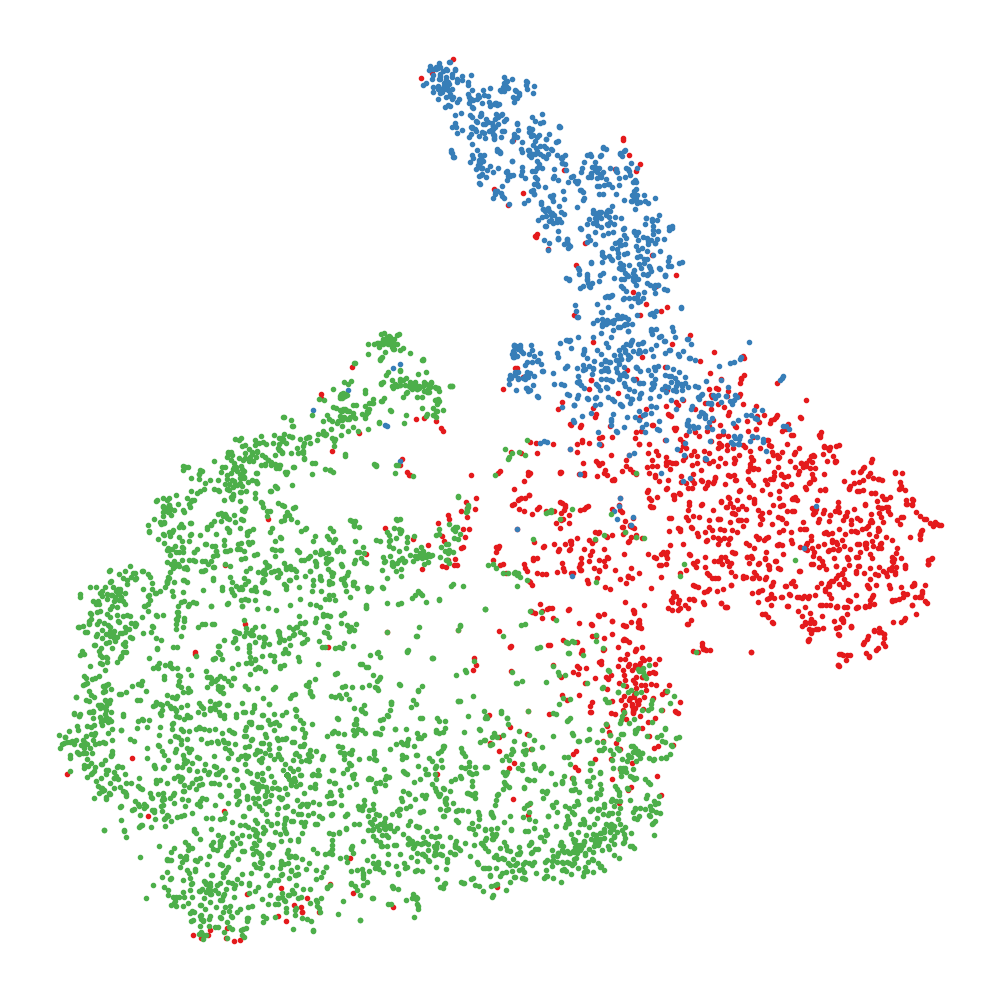
\includegraphics[width=4.04cm]{pic/chapter3/ober/tSNE-DP.png}
  }

  \subfloat[]{
    
\includegraphics[width=7.04cm]{pic/chapter3/ober/tSNE-label.png}
  }
  \caption{E-SAR Oberpfaffenhofen地区数据地区数据不同方法特征分布。(a) CNN-T; (b) CNN-P; (c) CNN-F; (d) CNN-SE; (e) CNN-CBAM; (f) 本章方法}
  \label{fig:ober-tSNE}
\end{figure}

表\ref{tab:ober_res}展示了各个方法的分类数值结果。本章提出的基于双通道注意力的极化信息提取方法总体准确率达到94.6\%,相比于其他验证方法提升了3.73\%。本章方法的散射特征时,在建筑物区域的分类准确率仅为63.16\%,这可能是因为建筑物区域目标散射回波差异性大,导致仅使用散射特征时,不能完全表征建筑物目标的特性,进而导致在建筑物区域可分性较低。与仅使用目标分解特征相比,直接堆叠极化特征在平均准确率指标反而下降1.32\%,这可能是由于该方法仅仅是对两类的特征进行简单的堆叠,堆叠后的特征维数过高,分类模型对于高维特征输入无法有效利用两种不同类型特征间的主次关系。本章方法在总体准确率、平均准确率、Kappa系数等指标上均有提升,验证了本章方法能有效的提升极化特征的表征方式,提升分类准确度。

图\ref{fig:ober_conf_matrix}展示了本章方法分类结果的混淆矩阵可视化图。混淆矩阵的可视化结果显示本章方法在对角线上具有较高的主对角元素,说明在大多数类别上取得了良好的分类性能。

%TODO:
\begin{table}[ht!]
  \caption{E-SAR Oberpfaffenhofen地区数据分类数值结果(\%)}
  \label{tab:ober_res}
  \begin{tabular}{cccccccc}
    \toprule[1.5bp]
    序号                        & 类别    & CNN-T          & CNN-P & CNN-F & CNN-SE & CNN-CBAM       & 本章方法           \\
    \midrule[0.75bp]
    1                         & 建筑    & \textbf{96.68} & 83.9  & 80.1  & 80.42  & 83.92          & 90.96          \\
    2                         & 林地    & 83.35          & 91.99 & 90.5  & 92.44  & 91.61          & \textbf{92.45} \\
    3                         & 开放区域  & 89.83          & 90.04 & 91.37 & 91.63  & 91.41          & \textbf{96.89} \\
    \midrule[0.75bp]
    \multicolumn{2}{c}{OA}    & 89.56 & 88.97          & 88.52 & 89.13 & 90.27  & \textbf{94.6}                   \\
    \multicolumn{2}{c}{AA}    & 89.95 & 88.64          & 87.32 & 88.16 & 89.98  & \textbf{93.43}                  \\
    \multicolumn{2}{c}{Kappa} & 81.63 & 83.51          & 82.73 & 83.58 & 85.24  & \textbf{90.78}                  \\
    \bottomrule[1.5bp]
  \end{tabular}
\end{table}

\begin{figure}[ht!]
  \centering
  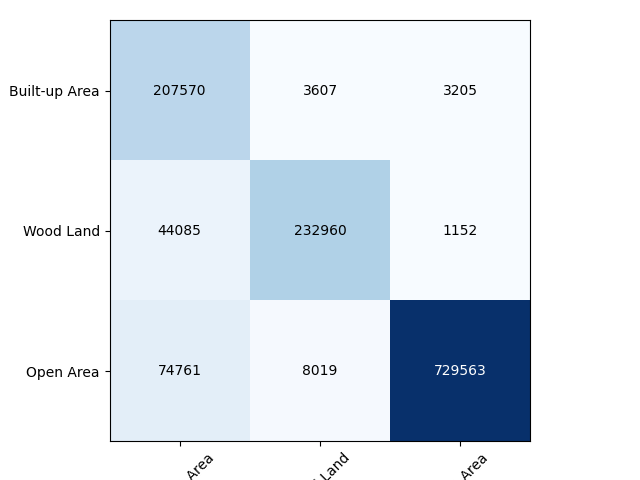
\includegraphics[width=10.4cm]{pic/chapter3/ober/conf-matrix.png}
  \caption{本章方法在E-SAR Oberpfaffenhofen图像中分类结果混淆矩阵图}
  \label{fig:ober_conf_matrix}
\end{figure}



\section{本章小结}
本章针对极化ASR图像信息利用中所面临的信息冗余问题,提出了一种基于双通道注意力的极化信息提取方法。通过构建极化散射特征通道和目标分解特征通道的双通道结构,结合空间、通道注意力机制,能够有效地提取出两种不同类型的极化特征中的关键极化信息。为了增强两种信息的关联,设计了散射特征导向的注意力修正方法,对注意力权重进行修正,从而全面聚合关键极化信息。最后设计多尺度特征学习模块,赋能模型对不同尺度极化信息的捕捉能力。最后通过视觉和数据量化两个层面进行性能评估,结果表明本章提出的方法能够有效地提升极化数据中的信息表征方式,从而提升极化SAR图像的分类精度。